\chapter{SKA1-mid Multiband Primary Beams: Effects of HI and CO Intensity Mapping Experiments} % Main chapter title
% INVESTIGATING INTENSITY MAPPING EXPERIMENTS WITH SKA1-MID PRIMARY BEAMS 
\label{Chapter6} % For referencing the chapter elsewhere, use \ref{Chapter1} 

\textbf{Overview}\\
\par\noindent\rule{\textwidth}{0.4pt}\\
 \textit{This Chapter introduces us to the SKA1-mid instrument and describes how we generate the beam patterns of Bands $1, 2$ and $5$ using the {\tt GRASP} software package.
 Zernike models of these beams for the various bands are produced  and used to investigate the effects of CO and HI intensity mapping.
%  is a measure of how numerically stable the true polarization can be recovered from measured antenna voltages.\ldots
% the simulation methods utilized in the numerical study of the
% reflector antenna systems with the Eleven antenna feed. The methodology and theory are introduced in Section 4.1. 
% The specification details of simulations performed in TICRA’s software {\tt GRASP} 9 [31] are presented in Section 4.2. 
}
\par\noindent\rule{\textwidth}{0.4pt}\\


%%
\section{Introduction}	  \label{chap6:intro}
%%

%%
% \subsection{The Design of SKA1-mid}	  \label{chap6:ska1-mid}
%%
SKA1-mid is currently being assembled in South Africa and forms part of the three interferometric array of the SKA \citep{2018AAS...23121503S,8105424,vermij2014exascale}. The instrument is designed to have $197$ parabolic dishes (with $64$ MeerKAT dishes inclusive) and a maximum baseline of $150 \, \rm km$. The feed design of the dishes will be a single-pixel with a total number of $254$ \citep{vermij2014exascale} and it will have the ability to capture signals within five different bands between $0.35 \, \rm GHz$ to $13.8 \, \rm GHz$. The design topology of this instrument is to have $\sim 1\, \rm km$ diameter of dense inner elements and a randomly dispersed offset dishes in a spiral shape as shown in Fig.~\ref{fig:ska1-mid}. Refer to \citep{2018arXiv180511455S} to understand the technical details in Fig.~\ref{fig:ska1-mid}.
%%%
\begin{figure}
\begin{minipage}[H]{\linewidth}
\centering
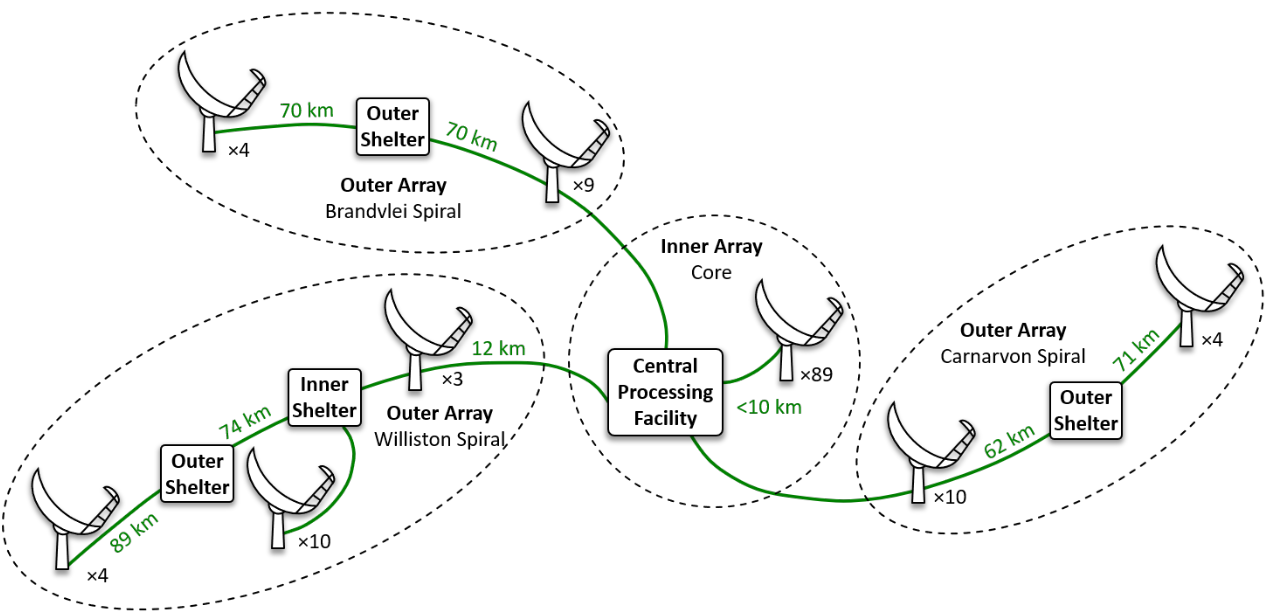
\includegraphics[width=\linewidth]{c6/ska1-mid}
\caption{\label{fig:ska1-mid} 
\enquote{Layout of the planned SKA1-MID telescope showing the locations of the antennas in the core and in the three spiral arms} (Fig.~\ref{fig:ska1-mid} and the caption are obtained from \citep{2018arXiv180511455S}).}
   \end{minipage}
\end{figure}
\FloatBarrier


\noindent \enquote{This telescope will primarily address observations of radio pulsars and observations of the 21 cm hyperfine line of neutral hydrogen from the local Universe, to moderate redshifts, as well as high
sensitivity observations of continuum emitting objects. It will also be well suited for conducting
observations of various spectral lines in addition to the 21-cm hydrogen line (e.g. OH-lines), many classes
of radio transients, magnetized plasmas both in the Galaxy and intergalactic space, and potentially protoplanetary disks}
\citep{dewdney2015ska1}.


Although this instrument is not exclusively designed for IM experiments, it will be good to investigate its 
potential for this technique, especially for Bands $1$, $2$ and $5$ receivers which fall within the permitted budget of SKA1-mid. For further details on the description and classification of SKA1 system refer to \citep{chai2016experiments,dewdney2015ska1}.


%%
%  \subsection{Line Intensity Mapping}	 \label{chap6:line-im}	
%%  of carbonmonoxide (CO),
% The technique employed in the IM experiments is to use the integrated emission from spectral lines in galaxies and /or
% diffuse IGM to track the growth and evolution of cosmic structure. This is essential to understand the spatial 
% fluctuations in the line emission from many individually unresolved galaxies, rather than targeting galaxies one by one. 
% Currently, dozens of research on IM as stated in Chapter \ref{Chapter1} promise new insights into the evolution of the Universe at low redshifts 
% and into the Epoch of Re-ionisation and Cosmic Dawn at high redshifts. The most general spectral line discussed is the 21 cm neutral hydrogen line.
% However, other lines trace different physical processes, and some lines may be easier to study, either because they are
% brighter or they appear in a less difficult frequency band. Thus, it is useful to study other lines in addition to the 21 cm
% line. Some other lines which have been proposed include 
Here, we investigate the IM of CO line (for high redshift) in addition to HI at low redshift, particularly focusing on the observational effects of primary beam distortion of the SKA1-mid for Band $1$ (i.e. $350 - 1050$ MHz), Band $2$ (i.e. $950 - 1760$ MHz), Band $5a$ (i.e. $4.5 - 8.4$ GHz) and Band $5b$ (i.e. $8.4 - 13.6$ GHz). CO is a powerful tool to detect atomic gas and star formation in immediate galaxies and also, the most dominant molecular species after H\textsubscript{2}.

Next, we describe how we use the EM simulator to produce the primarily beams of SKA1-mid. 
% tracing the metal-enriched, relatively dense ($\gtrsim 10^2 $ cm\textsuperscript{-3})
% specifically, to study the feasibility of a CO intensity mapping survey targeted at $z \sim 5$, using the SKA1-mid primary beams.
% However, .....
% 
% Intensity mapping can be performed using many different spectral lines. The most commonly discussed is the 21
% cm neutral hydrogen line. 

\let\cleardoublepage\clearpage

%%
\section{{\tt GRASP} Beam Measurement}			  \label{chap6:em}
%%

{\tt GRASP} software is a commercial package used to design and analyse single and dual reflector telescopes as well as multi-reflector and multi-feed antennas. This section concentrates on the physical geometry and EM methods applied for the SKA1-mid analysis. A complete description of the package with mathematical expressions of the geometries and EM models as well as output data capabilities is given in the {\tt GRASP} Technical Description, which may be retrieved from the Help Menu.
% and antenna farms. Single and dual reflector antennas, multi-reflector
% and multi-feed antennas, as well as gridded and shaped reflector antennas can be set-up and analyzed. Reflector imperfections can be considered by
% including thermal and mechanical distortions, gaps between reflector panels, supporting struts and scatterer material properties.
%%
\subsection{Model Specification}	  		\label{chap6:mspec}
%%
% The simulation environment setup of the reflector and feed models is described in this section.
Here, we setup the actual geometry of the instrument.

%%
\subsubsection{Reflector Antenna Models}		  \label{chap6:rspec}
%%%

Fig.~\ref{fig:geo-model} illustrates the dual reflector design of SKA1-mid. It includes an offset paraboloidal main reflector and a sub-reflector, with the principal focus hosting the receiver. Note how the receiving rays bounce off from the main dish to the secondary reflector and then finally go into the feed. This can be achieved by manually defining the following parameters:
%%%
\begin{figure}
\begin{minipage}[H]{\linewidth}
\centering
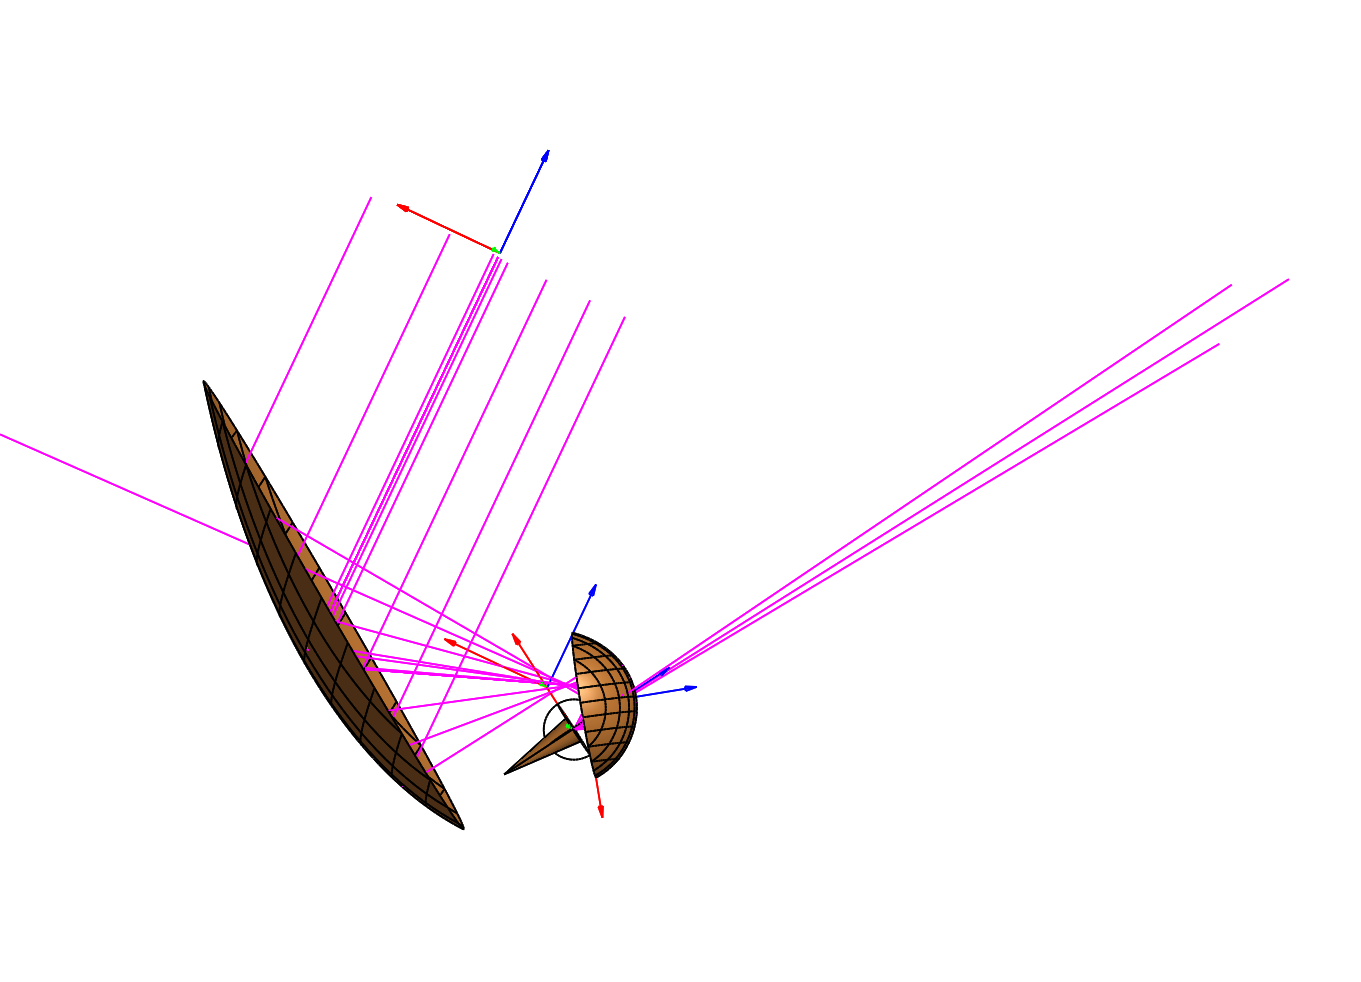
\includegraphics[width=\linewidth]{c6/image3D}
\caption{\label{fig:geo-model} A geometrical dual reflector model of SKA1-mid oriented in the $xz-$ direction and generating highly contoured beam.}
   \end{minipage}
\end{figure}
\FloatBarrier
%%

\begin{itemize} %{enumerate}
 \item focal length of the reflector;
\item angle between the axis of the primary reflector and the sub-reflector;
\item focal distance for the sub-reflector;
 \item eccentricity for the sub-reflector;
 \item angle between the axis of the secondary reflector  and the feed;
\item  aperture diameter of the main reflector;
 \item the wavelength of the operating frequency. 
\end{itemize}%{enumerate}
%%

% \noindent Either these parameters may be entered directly by the user or automated by means of the mouse. The automation will control the
% position of the feed and allow the user to obtain a wide range of designs in a flexible manner by altering the values of the parameter's
% angle  and the focal distance. 
% %%
% 
% When these parameters are provided, the design is constructed in the following way: the central ray
% from the feed, the direction of which is defined by the angles from the main reflector axis to the sub-reflector axis and 
% from the sub-reflector axis to the feed axis, is reflected from the sub-reflector and hits the main reflector at a point which is selected as the centre for
% the circular main reflector aperture.
% %%


%%
\subsubsection{Feed Models}				  \label{chap6:feedspec} 
%%

The feed system used in this chapter is an aperture illumination of the antenna system and this is possible in a receiver situation. A general way to represent the illumination from a feed is through tabulated data from its beam pattern, which may come from measurements or calculations. The beam pattern of the feed used in the analysis is the measured far-field pattern, which consists of received fields in $\theta, \phi \rm -plane$
($\theta, \phi$ define the field point on a sphere). 
%
%% 	+++++++++++++++++++++++++++++++++++++++++++++++++++++++++++++++++++++++++++
\section{Modelling EM Beams}   \label{chap6:mdling}
The {\tt GRASP} software used to produce the EM beams considers the basis of physical optics (PO) together with the physical theory of diffraction (PTD). The simulations are made for Bands $1, 2$ and $5$. For the purpose of this work, we present a 2D grid for the simulated beams at $450 \, \rm MHz$, $990.5 \, \rm MHz$ and $4.6 \, \rm GHz$ as shown in the first rows of Figs.~\ref{fig:band1}, \ref{fig:band2} and \ref{fig:band5a} independently. These beams are presented in the Jones matrix (XX\footnote{{\tt Horizontal linearly unpolarized beam}}, XY\footnote{{\tt Horizontal linearly polarized beam}}, YX\footnote{{\tt Vertical linearly polarized beam }}, YY\footnote{{\tt Vertical linearly unpolarized beam}}) and we can clearly observe from the gain components (XX and YY) that at lower frequencies particularly, for Band 1, we have a wider field-of-view (with less or no side-lobes) as compared to higher frequencies (with more side-lobes) as that of Band 5. Generally, in all parabolic reflectors, observing at higher frequencies produce narrower beam widths and therefore, it is just obvious that the Band 5 beam widths are much narrower than the lower bands (1 and 2). Nevertheless, such a beam width entails specifically, accurate dish surface regularity along with strong pointing accuracy. 
Understanding this primary beam effect is very significant in IM experiment since the technique involves multiple pointing in the sky in order to estimate the total intensity.

With the aim of investigating IM experiment with the SKA1-mid, we try to model the simulated beams, using Zernike polynomials (ZP) discussed in Chapter~\ref{Chapter5}. After that, we introduce errors in the physical geometry of the instrument and finally, use these beams to simulate the foreground examined in Chapter~\ref{Chapter3}.
% , we try to reconstruct the {\tt GRASP} beam models using Zernike fits and also, introduce errors in these {\tt GRASP} beams for IM experiments.

\subsection{ Fitting 2D Zernike Polynomials on EM Beams}	  \label{chap6:zern}
%https://github.com/kmbasad/eidos

The mathematical basis of ZP is discussed extensively in Chapter~\ref{Chapter5}. In this section, we repeat the same approach, using the appropriate radial order
to reconstruct the beams to display both the spatial and spectral representations of the EM beams. 

%   
\subsubsection{Spatial Representation}	  \label{chap6:zspatial}
%
The reproduction of the EM beams for channels 450 MHz, 990.5 MHz and 13.6 GHz, depend on the upper limit of Zernike modes (angular frequencies) to use. This maximum number defines the strongest modes necessary for extracting features from the simulated beams. Fig.~\ref{fig:nmodes} shows the mean square error (MSE) plots needed to choose the maximum number of modes\footnote{{\tt Nmodes is computed as $ n+1 + \sum range(n+1)$, n is the radial order.}}. For instance, to reconstruct the unpolarized components (XX and YY) of the beams at 450 MHz, we choose an upper limit of $56$ modes as shown in Fig.~\ref{fig:xx} (blue plot). The same number of modes is selected (refer to Fig.~\ref{fig:xy} (blue plot)) if we want the basis functions to model the cross terms (XY and YX). Note that these $56$ modes of ZP are obtained from an n-order (radial index) of $10$. Similarly, taking the beams at the next two channels (990.5 MHz and  13.6 GHz), we select $100$ modes (orange plot) and $150$ modes (green plot) in Fig.~\ref{fig:xx} to model the diagonal parts. After that, we select the same number of modes (100 and 150) in  Fig.~\ref{fig:xy} to describe the cross terms.  These MSE plots, clearly show that if we increase the number of modes other than what we have chosen, there would not be any significant variation  in  the reconstructed beams.

Next, the corresponding coefficients can be computed, using Equation~\ref{eq:invmthd2}. Now, having the strongest coefficients ($\bm{C_{\rm k}}$) and the strongest basis functions ($\bm{\eta_{\rm k}}$), we reconstruct the simulated beams ($\bm{R_{\rm \Phi}}$) as:
%%
\begin{equation}\label{eq:R}
\bm{R_{\rm \Phi}} = \sum\limits_{k=0}^{N^m} \bm{C_{\rm k} \eta_{\rm k}}
\end{equation}

%%

\begin{figure}
%%
\centering
 \begin{minipage}[H]{\linewidth}
\begin{subfigure}[b]{0.8\textwidth}
      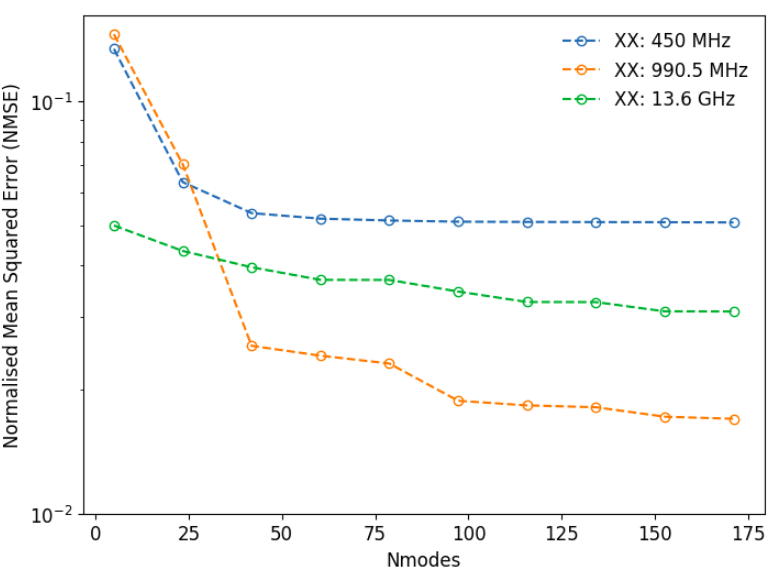
\includegraphics[width=\textwidth]{c6/XX_co} %mse_xx}
                \caption{}
                \label{fig:xx}
        \end{subfigure}
        \qquad
        \begin{subfigure}[b]{0.8\textwidth}
         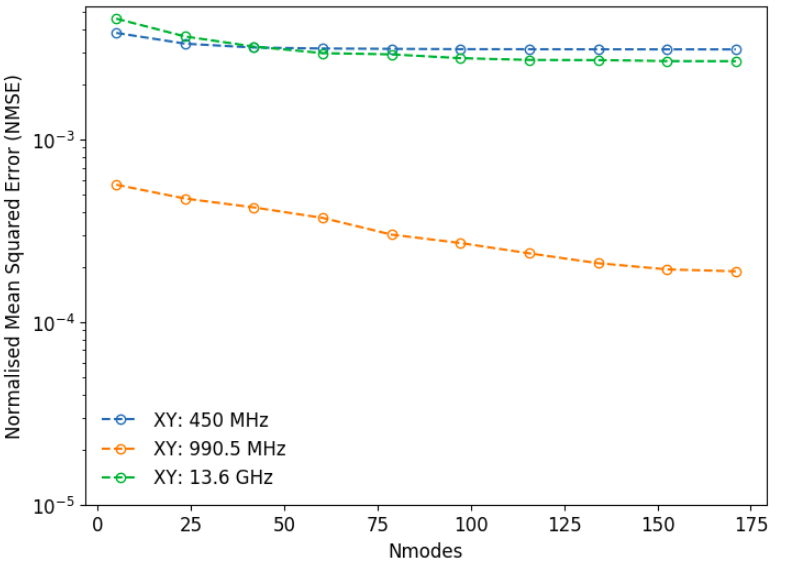
\includegraphics[width=\textwidth]{c6/XY_co} %mse_xy}
                \caption{}
               \label{fig:xy}
        \end{subfigure}
         \end{minipage}
    \caption{Representation of MSE for using the number of ZP at 450 MHz (blue), 990.5 MHz (orange) and 13.6 GHz (green).
    Panel (a) shows the gain term (XX) for each channel band whilst Panel (b) displays the cross term (XY). }
	    \label{fig:nmodes}
  \end{figure}
  \FloatBarrier
%%utmost

\noindent The second rows in Figs.~\ref{fig:band1}, \ref{fig:band2} and \ref{fig:band5a} show the Zernike beam models of $\bm{R_{\rm \Phi}}$ for Bands $1$, $2$ and $5$ respectively. These restored images clearly show that the Jones elements XX and YY can be represented using almost the same modes due to the similarities of the power coefficients in both cases. Similar explanations go for the off-diagonal elements. Moreover, the high number of modes used in the Band $5$ channel is due to the increase in the number of sidelobes. Note that an increase in the number of modes brings about a high radial order which is very important to model high sidelobes like in the case of Band $5$. Nervetherless, at lower frequencies, less or no side-lobes will be present within the same region, and hence, lower orders will dominate the model like in the case of Band $1$ and to some extend the lower channels of Band $2$.

% Band $1$ beams are reconstructed with the $10$ highest Zernike coefficients and that of Bands $2$ and $5$ can be reconstructed with the $40$ and $500$ 
% highest Zernike coefficients accordingly. The high value of coefficients in Band $5$ is due to the decrease in the beamsize 
% as a result of high antenna gain at high frequencies, making IM at this band very difficult since the radio telescope will require very careful control over its position.
% Hence, in modelling the Band $5$, we need at least $1000$ Zernike coefficients with corresponding basis patterns to choose the highest $500$ coefficients from.
After the reconstruction, the residual value obtained in the gain terms is $\approx 1 \%$ (for Bands $1, 2$ and $5$) and the cross terms, we have $ \approx 0.01 \%$ (for Bands $1, 2$ and $5$), showing that the proposed mathematical model in this case ZP, is good to consider when modelling beam patterns.
%%%
\begin{figure}
\begin{minipage}[H]{\linewidth}
\centering
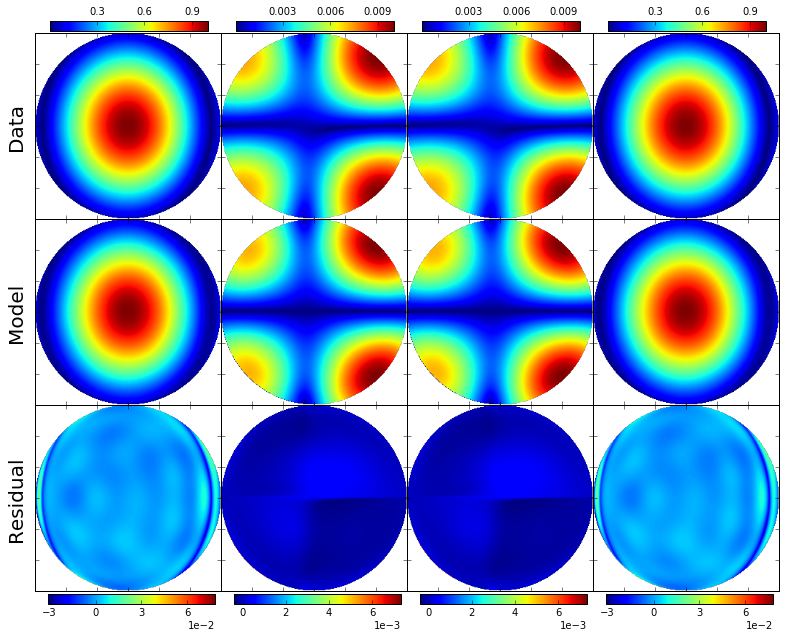
\includegraphics[width=\linewidth]{c6/spatial/zb1img}
\caption{\label{fig:band1} Top Row: Simulated EM model of SKA1-mid beam (in amplitude form) with a diameter of $6^\circ$ at $450$ MHz in a normalised unit. Middle Row: The restored model of the first row, using Zernike fit. Last Row: The respective beam errors between the top two rows.
Here, columns one and four are the amplitude beams of XX and YY respectively whilst the beams in the second and third columns are XY and YX correspondingly.}
\end{minipage}
\end{figure}
\FloatBarrier
%%


%%
\begin{figure}
\begin{minipage}[H]{\linewidth}
\centering
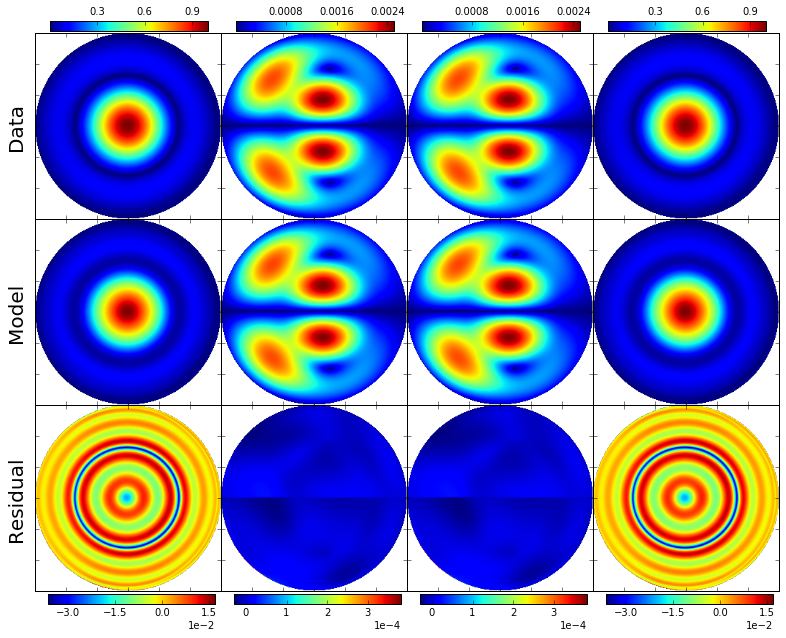
\includegraphics[width=\linewidth]{c6/spatial/band2a}
\caption{\label{fig:band2} Top Row: Simulated EM model of SKA1-mid beam (in amplitude form) with a diameter of $6^\circ$ at $990.5$ MHz in a normalised unit. Middle Row: The restored model of the first row, using Zernike fit.
Last Row: The corresponding beam errors between the 1\textsuperscript{st} two rows.
Here, columns one and four are the amplitude beams of XX and YY respectively whilst the beams in the second and third columns are XY and YX correspondingly.}
\end{minipage}
\end{figure}
\FloatBarrier
%%


%%
\begin{figure}
\begin{minipage}[H]{\linewidth}
\centering
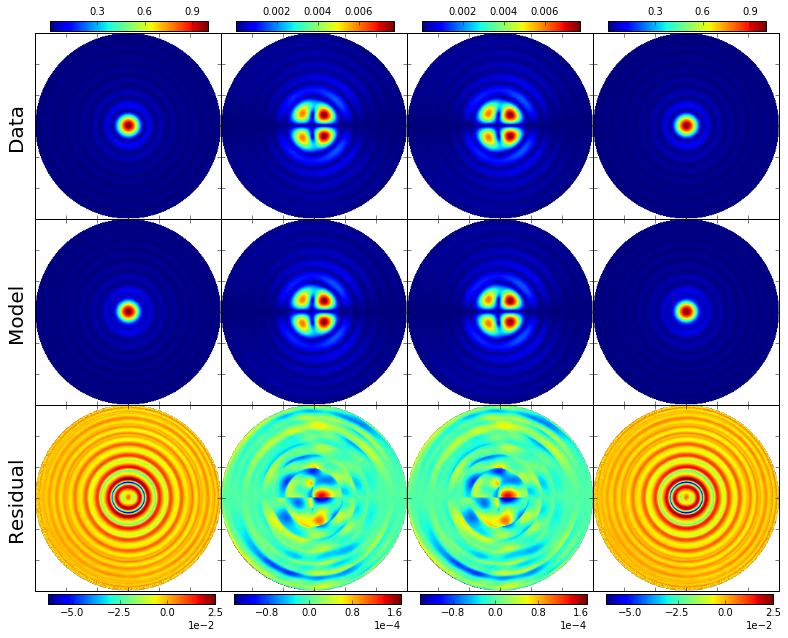
\includegraphics[width=\linewidth]{c6/spatial/band5a1}
\caption{\label{fig:band5a} Top Row: Simulated EM model of SKA1-mid beam (in amplitude form) with a diameter of $4^\circ$ at  $13.6$ GHz in a normalised unit. Middle Row: The restored model of the first row, using Zernike fit. Last Row: The corresponding beam errors between the 1\textsuperscript{st} and 2\textsuperscript{nd} rows. Here, columns one and four are the amplitude beams of XX and YY respectively whilst the beams in the second and third columns are XY and YX correspondingly.}
\end{minipage}
\end{figure}
\FloatBarrier
%%

\subsubsection{Spectral Representation}	  \label{chap6:zspectral}
%

Here, instead of fitting the Zernike model on a specific channel like we did in Section~\ref{chap6:zspatial}, the technique is applied on all the frequencies for all the  bands in order to understand the beam behaviour across the frequencies and more importantly, interpolate for any missing channels and reconstruct the beams
within Bands 1, 2 and 5. This can easily be done by generating the Zernike coefficients for these bands. This section presents spectra plots showing the strongest coefficients that is common in  full polarization components (XX, XY, YX and YY) of all the channels for all the bands. 
The spectra plots displayed from Fig.~\ref{fig:band1spec} to~\ref{fig:band5bspec} show that at lower wavelengths the ripple effect is much less than the higher ones, since the ripple must be in the order of wavelength. These plots are produced from the highest $6$ Zernike coefficients for Bands $1,2$ and $5$. The $Z_{\rm j}$ indexes in the legends are the Zernike basis functions in single modes. 
%%


%%
\begin{figure}[H]
\centering
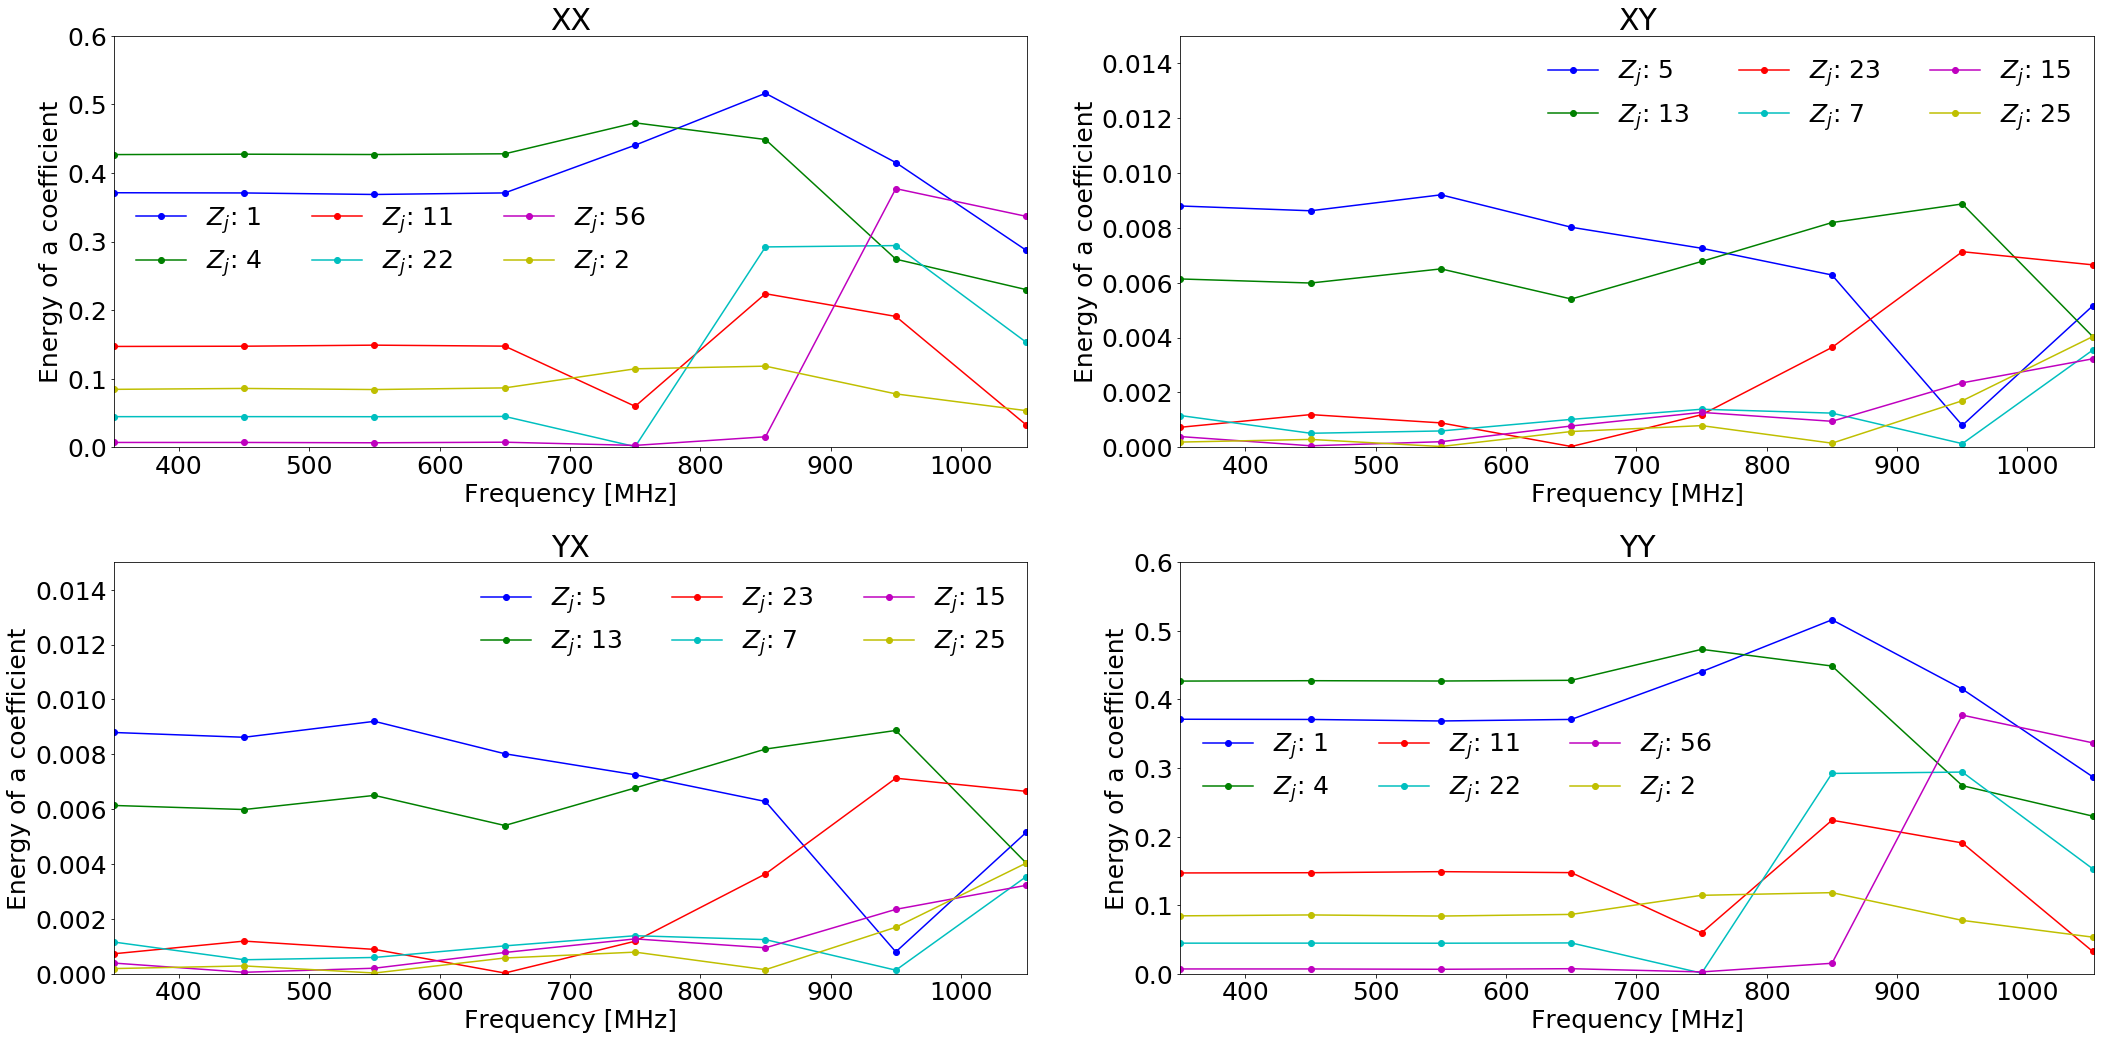
\includegraphics[width=\linewidth,angle=0]{c6/spectral/cf/band1_1050n} % [width=14cm, height=8cm]
\caption{\label{fig:band1spec} Spectral profile showing the various energy levels of Zernike coefficients for Band $1$ ($350 - 1050$ MHz).   The Zernike indexes (in the legends) are the activated basis functions that are frequent in all the channels.}
\end{figure}
\FloatBarrier
%%

%%
%%
\begin{figure}[H]
\centering
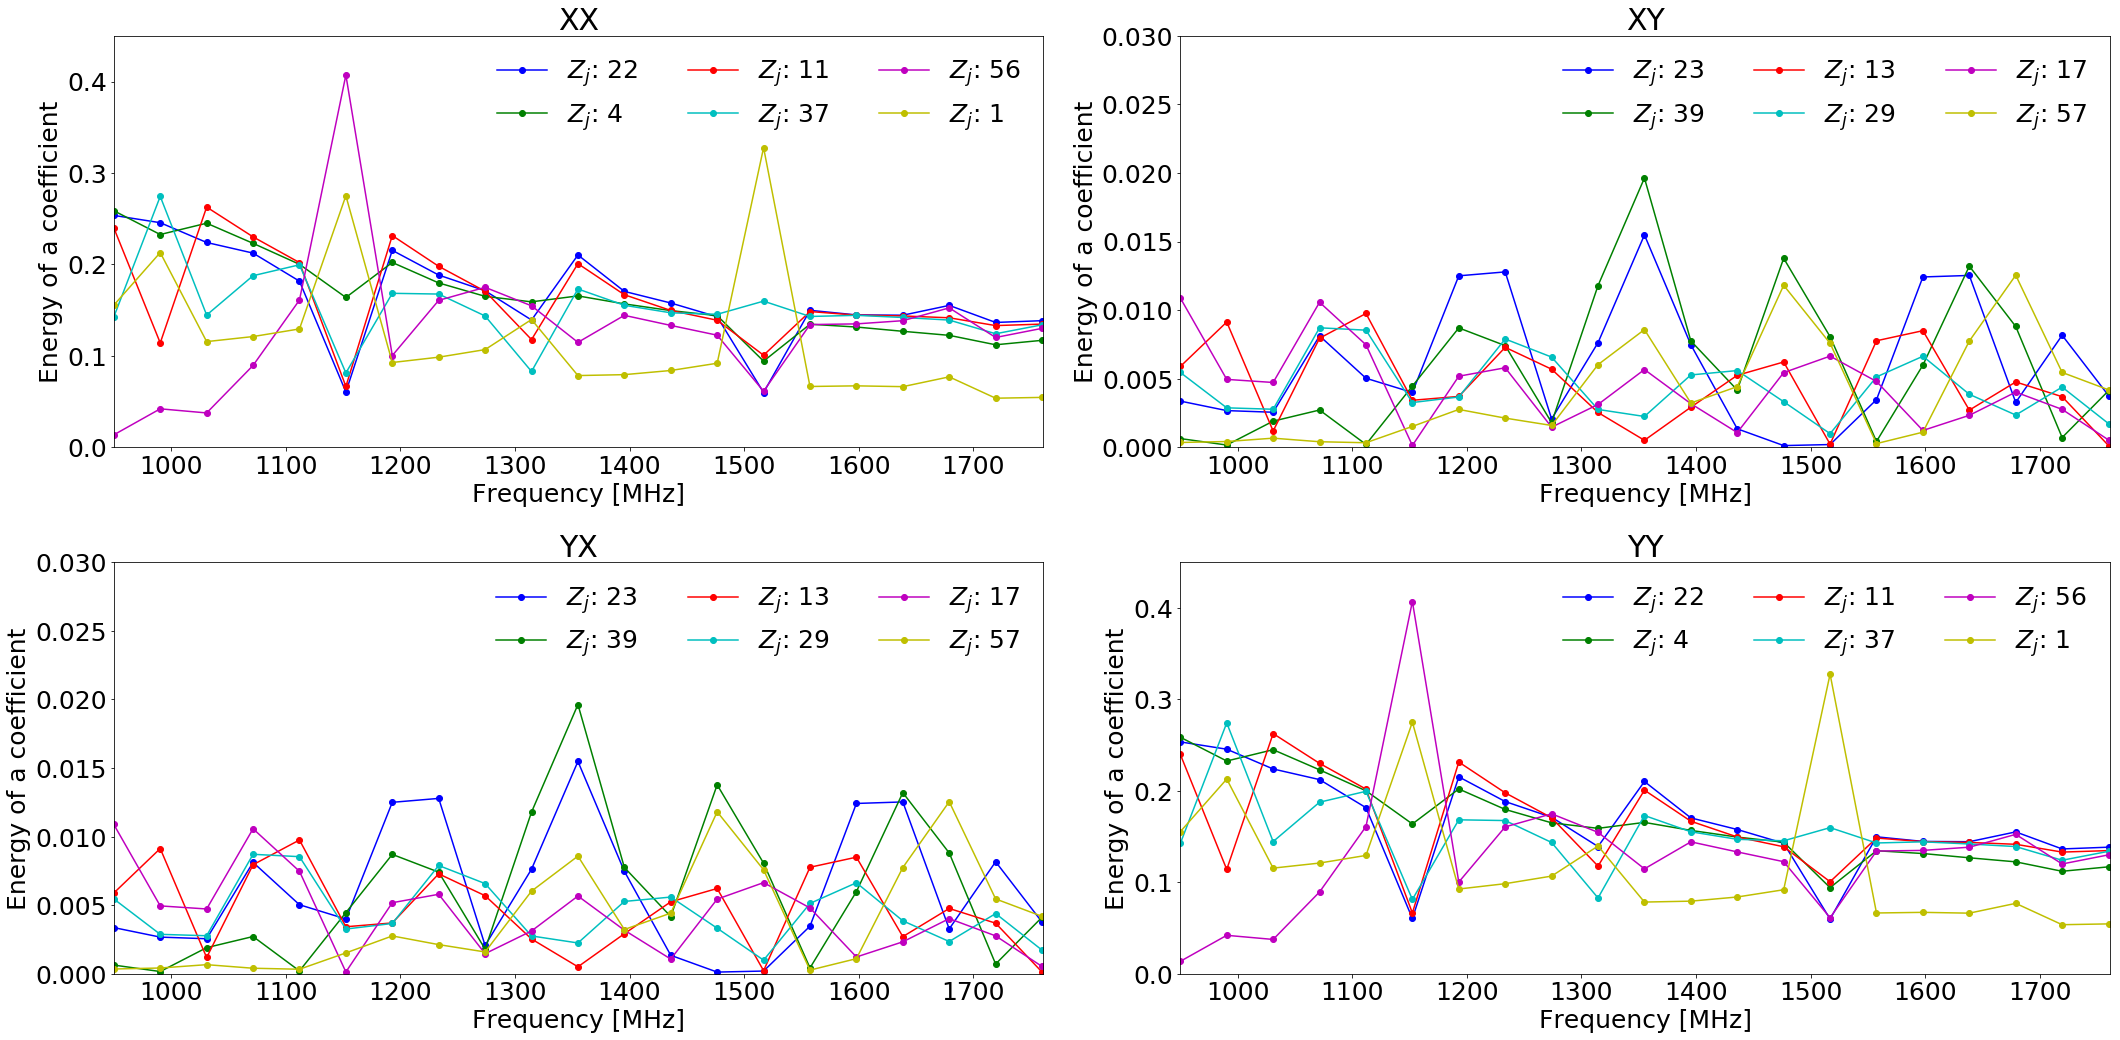
\includegraphics[width=\linewidth,angle=0]{c6/spectral/cf/band2_1760n} % [height=13cm, width=9cm]
\caption{\label{fig:band2spec} Spectral profile showing the various energy levels of Zernike coefficients for Band $2$ ($950 - 1760$ MHz).
The Zernike indexes (in the legends) are the activated basis functions that are frequent in all the channels.}
\end{figure}
\FloatBarrier
%%

%%
\begin{figure}[H]
% \begin{minipage}[H]{\linewidth}
\centering
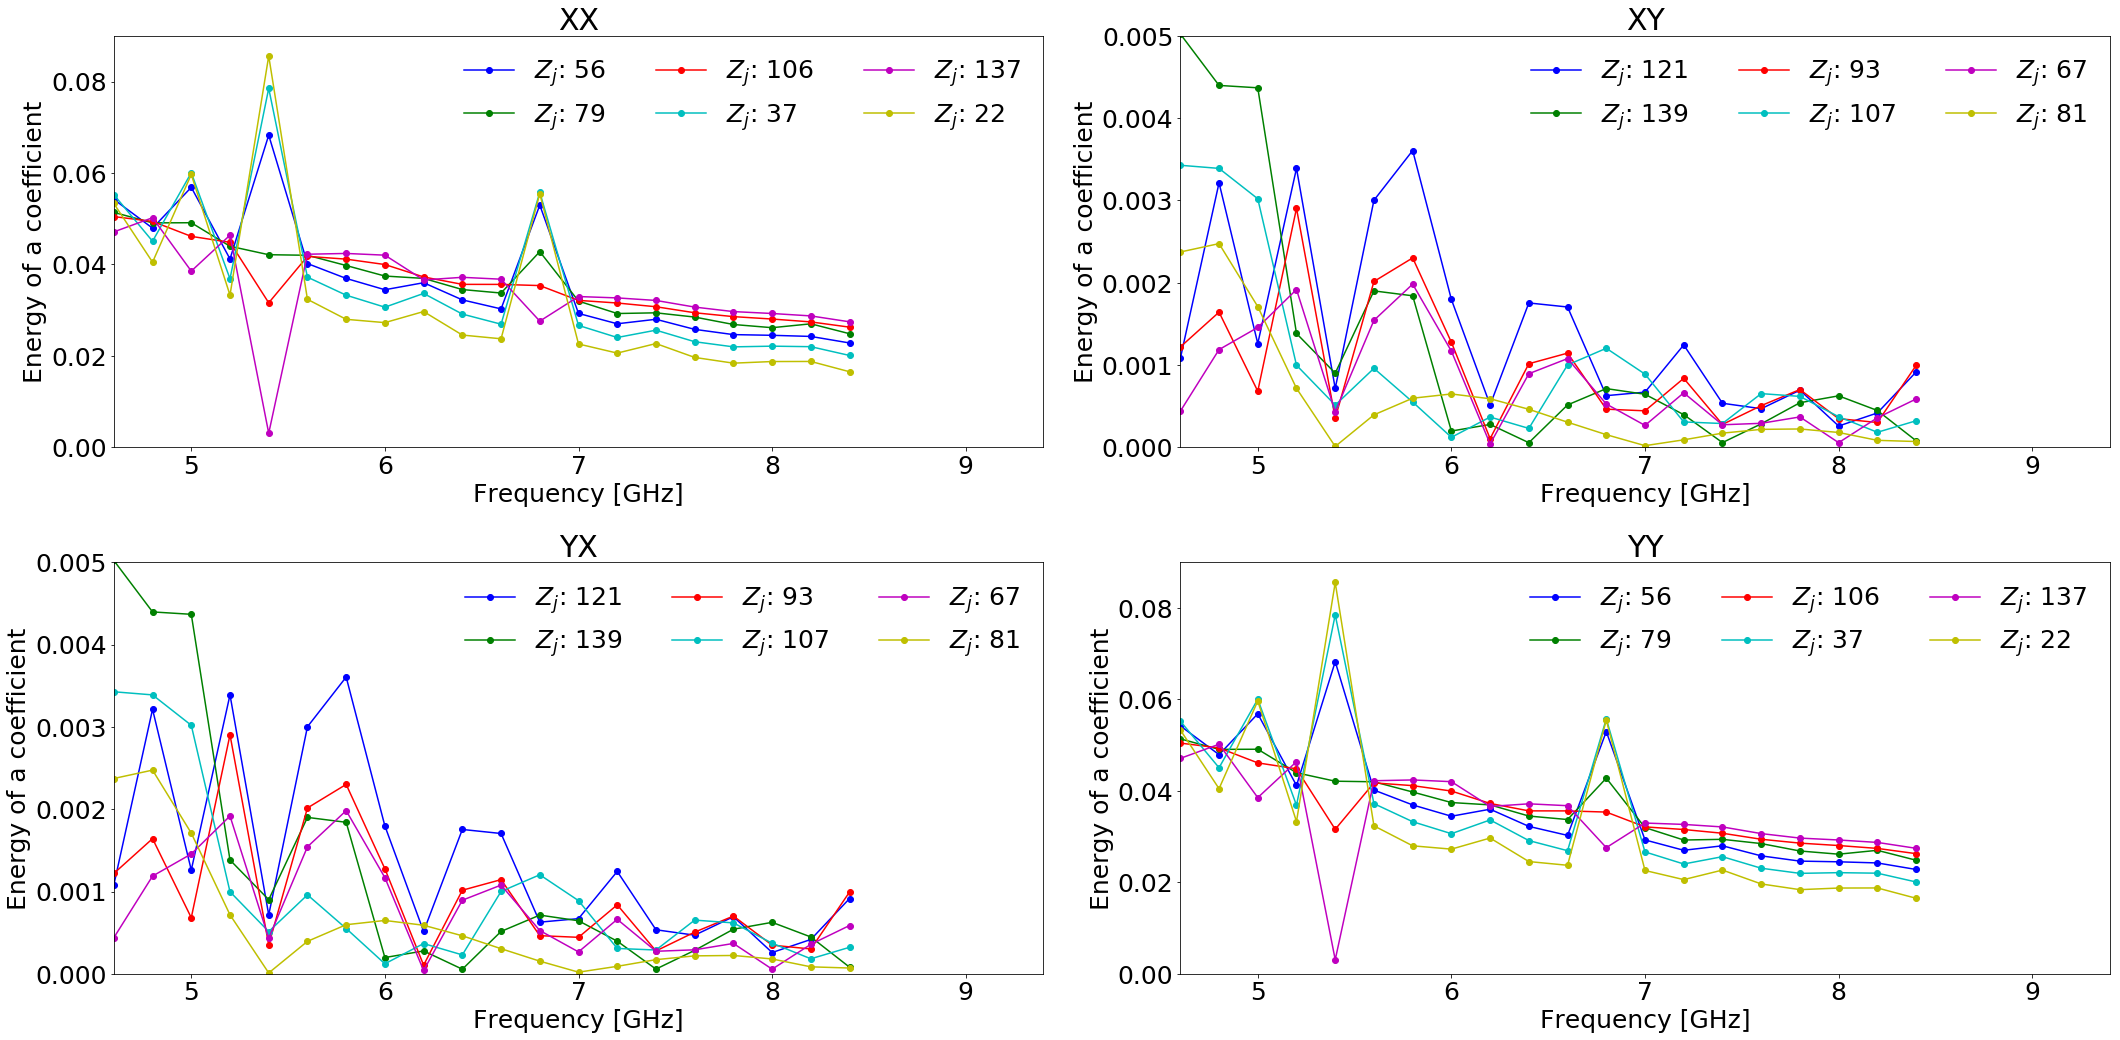
\includegraphics[width=\linewidth]{c6/spectral/cf/band5an}
\caption{\label{fig:band5an} Spectral profile showing the various energy levels of Zernike coefficients for Band $5a$ ($4.6 - 8.4$ GHz). The Zernike indexes (in the legends) are the activated basis functions that are frequent in all the channels.}
% \end{minipage}
\end{figure}
\FloatBarrier
%%

%%
\begin{figure}[H]
% \begin{minipage}[H]{\columnwidth}
\centering
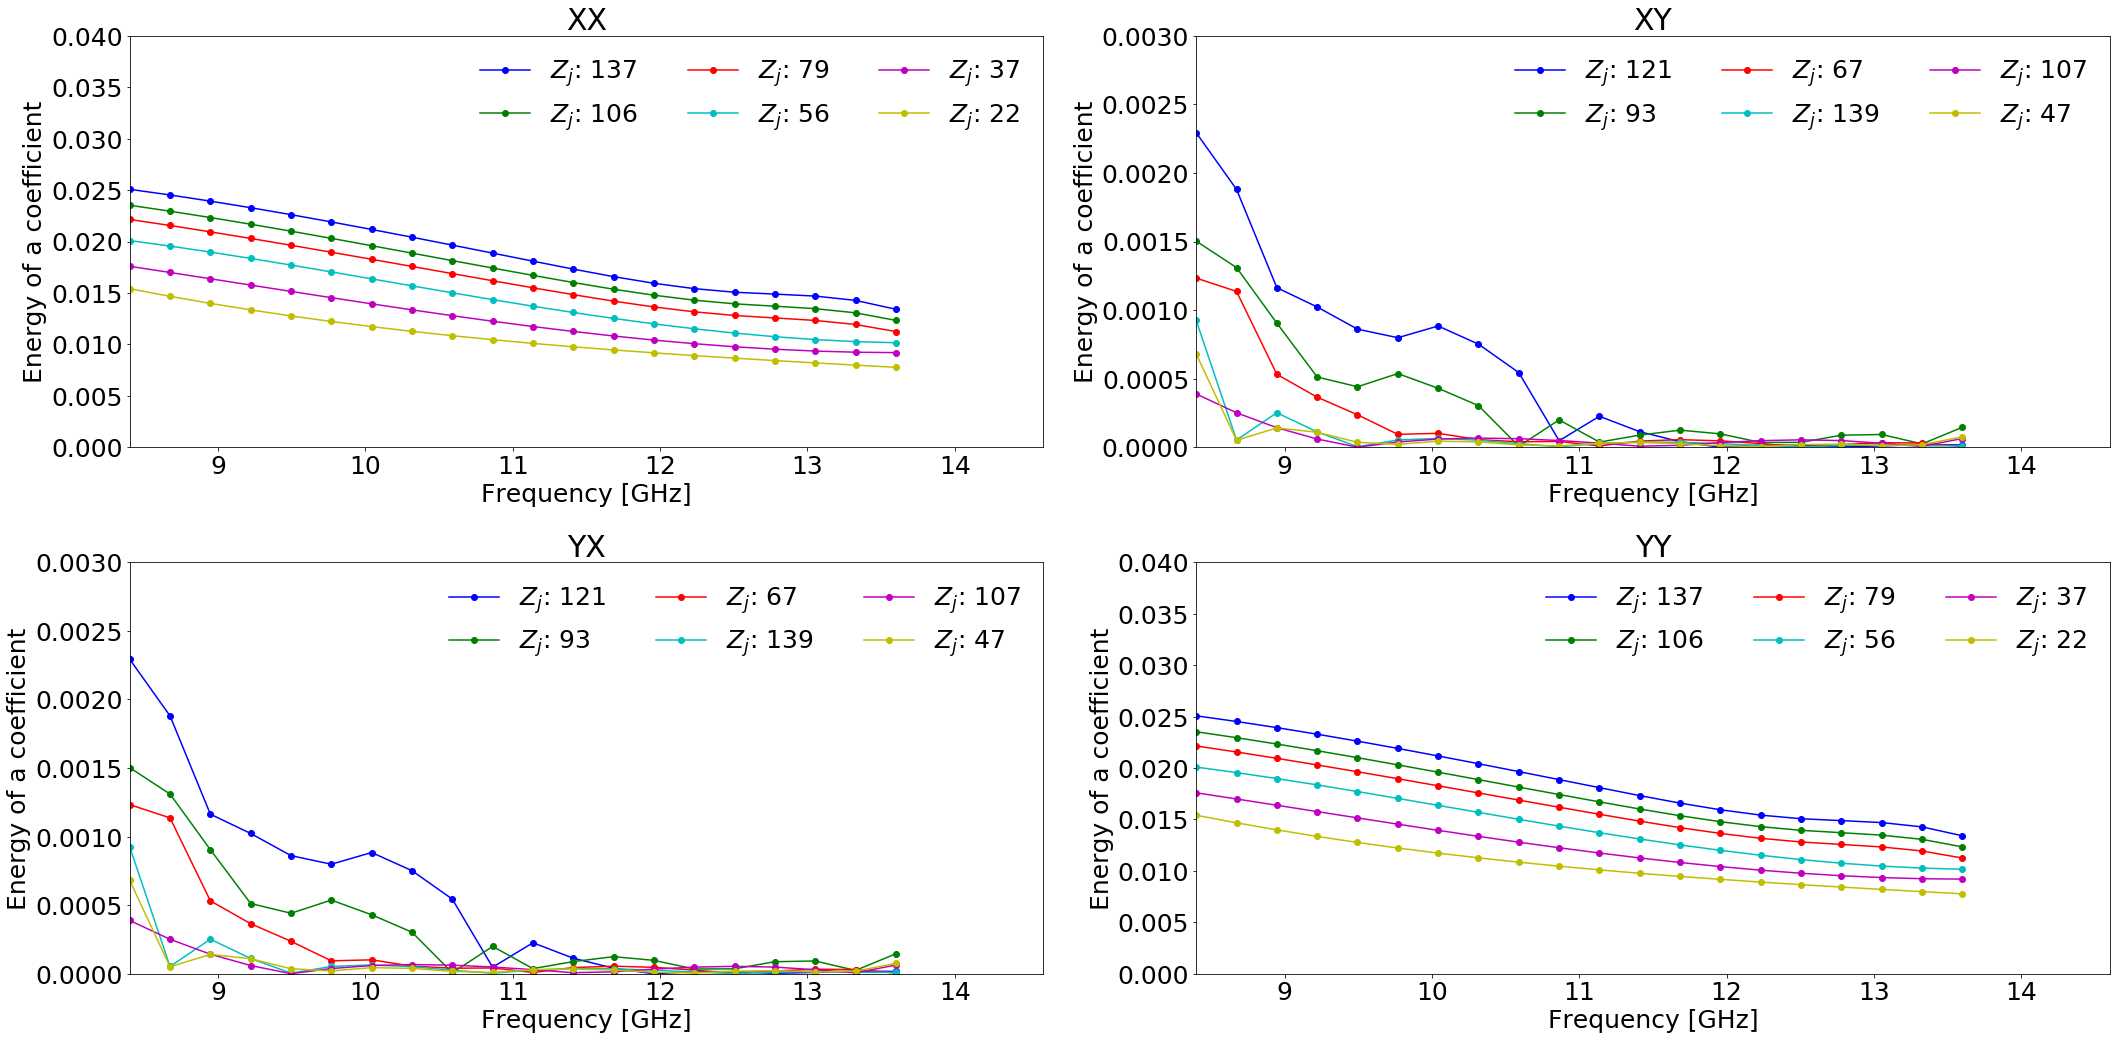
\includegraphics[width=\linewidth]{c6/spectral/cf/band5bn}
\caption{\label{fig:band5bspec} Spectral profile showing the various energy levels of Zernike coefficients for Band $5b$ ($8.4 - 13.6$ GHz). The Zernike indexes (in the legends) are the activated basis functions that are frequent in all the channels.} 
% \end{minipage}
\end{figure}
\FloatBarrier
%%

\noindent This is equivalent to the double index $Z_{\rm n}^{m}$ such that $n = ceil(-3/2 + \surd[9 + 8j]/2)$ and $m = 2j -n^2 - 2n$. For instance, in Band 1 (350 - 1050 MHz), $Z_{\rm 1} \longmapsto Z_{\rm 1}^{-1}, Z_{\rm 2} \longmapsto Z_{\rm 1}^{1}, Z_{\rm 4} \longmapsto Z_{\rm 2}^{0}, Z_{\rm 11} \longmapsto Z_{\rm 4}^{-2}, Z_{\rm 22} \longmapsto Z_{\rm 6}^{-4}, Z_{\rm 56} \longmapsto Z_{\rm 10}^{-8}$. We follow the same scheme to compute the double indexes for the other bands.


The next section presents how the {\tt GRASP} beams are corrupted.

\subsection{Model Beam Perturbation}	  \label{chap6:mbp} 
%%

Reflector imperfections can be considered by introducing thermal and mechanical distortions, gaps between reflector panels,
supporting struts and scatterer material properties. In this work, we displace the receiver from its focus to alter 
the aperture illumination pattern of the dish. This introduces a regular phase perturbations across the aperture and also,
a reduction in the signal gain. We can do this by adding regular phase error ($\sim 2^\circ$) in the beam-forming weight when generating the beams.
The effect of this beam distortion at 450 MHz, 990.5 MHz, and 13.6 GHz is represented in Figs.~\ref{fig:bandD1},  \ref{fig:bandD2}
and \ref{fig:bandD5a} respectively. Here, we note that there is a maximum error of $\approx 1\%$ in the residual plots (third row) of Figs.~\ref{fig:bandD1} and  \ref{fig:bandD2})
and $\approx 10\%$ error in Fig.~\ref{fig:bandD5a}. The high sensitivity of errors in the Band $5b$ beams (refer to the perturbed images in Fig.~\ref{fig:bandD5a}) 
confirms a reduction in the antenna directivity which is very crucial
in  IM experiments.
% This is because antennas operating at high frequencies, have shorter wavelengths
%%%
\begin{figure}
\begin{minipage}[H]{\linewidth}
\centering
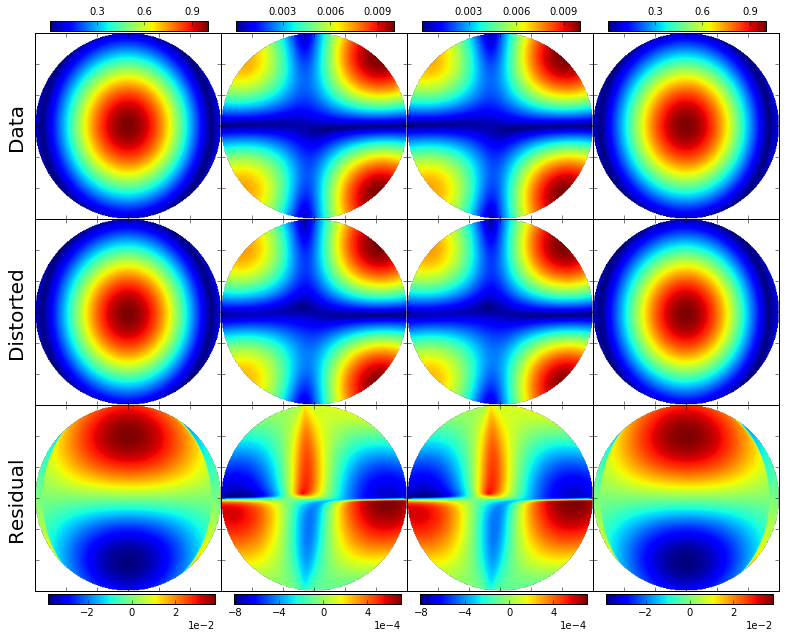
\includegraphics[width=\linewidth]{c6/distort-sim/beams/Dim1}
\caption{\label{fig:bandD1} Perturbed beams for Band $1$ at $450$ MHz. The data part (row 1) represents the original EM beams and the 
second row shows the corrupted EM beams due to systematic phase errors. The last row reports the differences between the respective beams in the top beams.  Note, the first and fourth columns are the amplitude beams of XX and YY respectively whilst the beams in the second and third columns are XY and YX correspondingly.}
\end{minipage}
\end{figure}
\FloatBarrier
%%

%%
\begin{figure}
\begin{minipage}[H]{\linewidth}
\centering
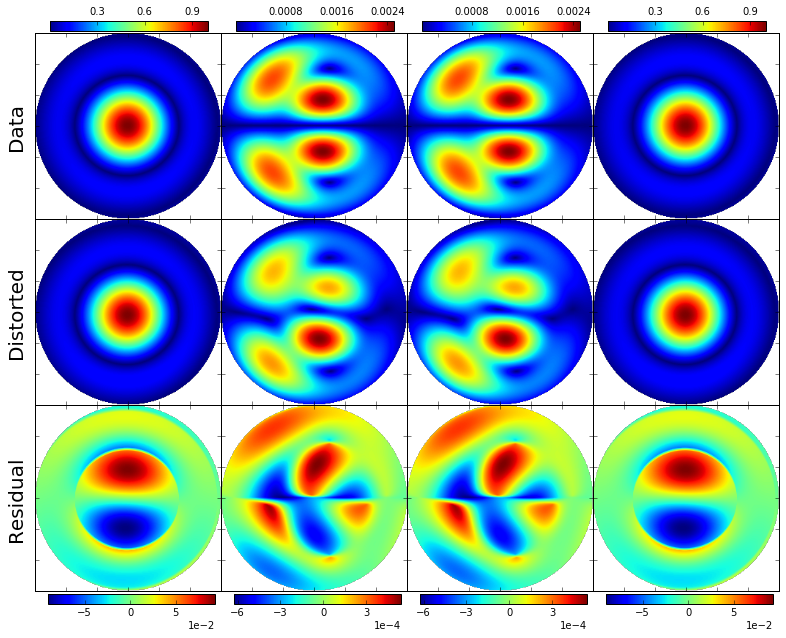
\includegraphics[width=\linewidth]{c6/distort-sim/beams/Dim2}
\caption{\label{fig:bandD2} Perturbed beams for Band $2$ at $990.5$ MHz. The data part (row 1) represents the original EM beams and the 
second row shows the corrupted EM beams due to systematic phase errors. The last row reports the differences between the respective beams in the top beams. Note, the first and fourth columns are the amplitude beams of XX and YY respectively whilst the beams in the second and third columns are XY and YX correspondingly.}
\end{minipage}
\end{figure}
\FloatBarrier
%%


%%
\begin{figure}
\begin{minipage}[H]{\linewidth}
\centering
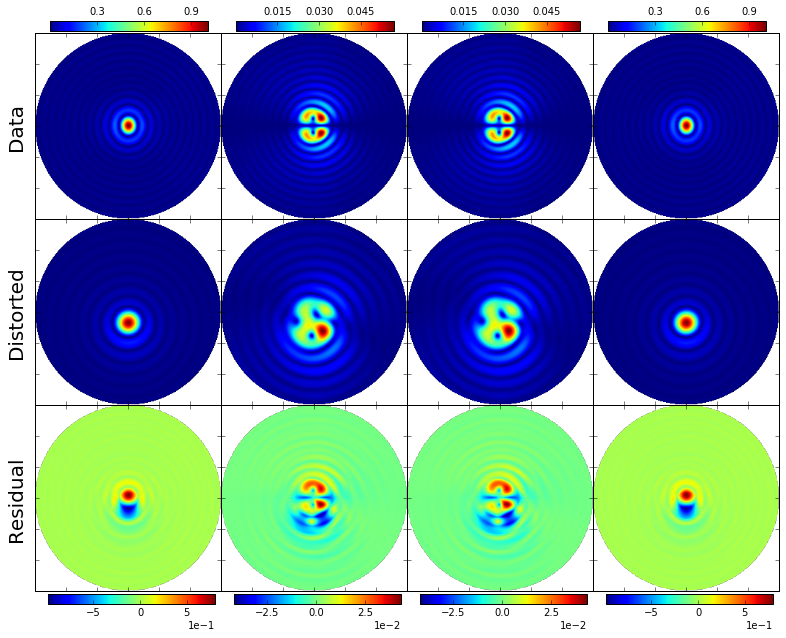
\includegraphics[width=\linewidth]{c6/distort-sim/beams/Dim5a}
\caption{\label{fig:bandD5a} Perturbed beams for Band $5$ at $13.6$ GHz. The data part (row 1) represents the original EM beams and the 
second row shows the corrupted EM beams due to systematic phase errors. The last row reports the differences between the respective beams in the top beams.
 Note, the first and fourth columns are the amplitude beams of XX and YY respectively whilst the beams in the second and third columns are XY and YX correspondingly.}
\end{minipage}
\end{figure}
\FloatBarrier
%%


\subsection{Intrinsic Cross-Polarisation (IXR)}	  \label{chap6:ixr} 
%%

Since the design of SKA1-mid is to operate in full polarization, it is therefore necessary to take measure of the performance of polarimetric. A common technique to do this is to use the intrinsic cross-polarization ratio (IXR) introduced in \cite{carozzi2011fundamental}.  \enquote{IXR is essentially the Jones matrix condition expressed as a cross-polarization ratio, and as such it is a measure of how numerically stable the true polarization can be recovered from measured antenna voltages} \citep{7303206}.

\noindent In this work, we are interested in Stokes polarimeters and so, the IXR is computed by converting the Jones matrix into Mueller matrix. Chapter~\ref{Chapter4}
discusses how the Mueller matrix is gleaned from the Jones formalism. 
%%
% figure of merit (FoM) to understand the polarization performance of a polarimeter is the intrinsic cross-polarization
% ratio (IXR) introduced by \citet{carozzi2011fundamental}. The term \enquote{intrinsic} in IXR indicates that the parameter is independent of the choice
% of coordinate systems. IXR is related to the invertibility of a DD Jones matrix. The Jones matrices are calculated by calibration and are inverted and multiplied with the data to give the 
% \enquote{corrected} data, and hence the intrinsic invertibility of a Jones matrix puts a fundamental limit to the extent to which data can be corrected. For Stokes polarimeters, 
% IXR can be easily converted to a Mueller IXR, which, in turn, is directly related to the fractional polarization leakage (fraction of Stokes $I$ signal 
% leaked into Stokes $Q, U, V$ and vice versa) caused by the beam, mathematically:
% 
%%
%\begin{figure}[ht!]
%    \centering
%    \begin{subfigure}{0.4\linewidth}
%        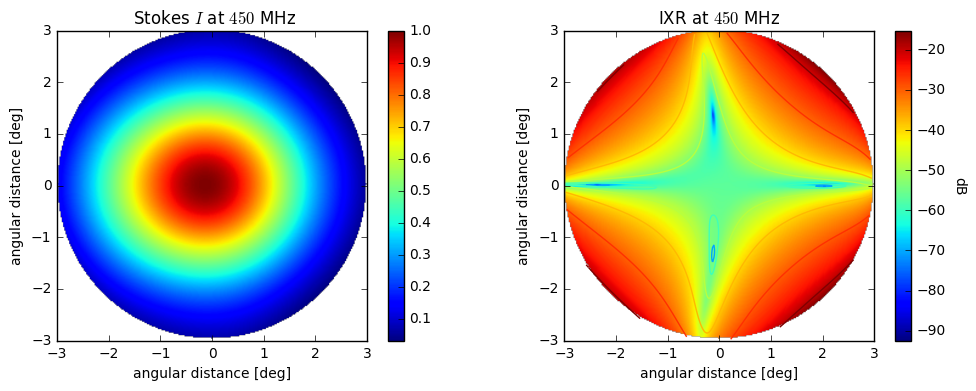
\includegraphics[scale=0.7]{c6/ixr/ixr_450mhz}
%        \caption{cc}
%    \end{subfigure}\\
%%    \hskip2em
%    \begin{subfigure}{0.4\linewidth}
%        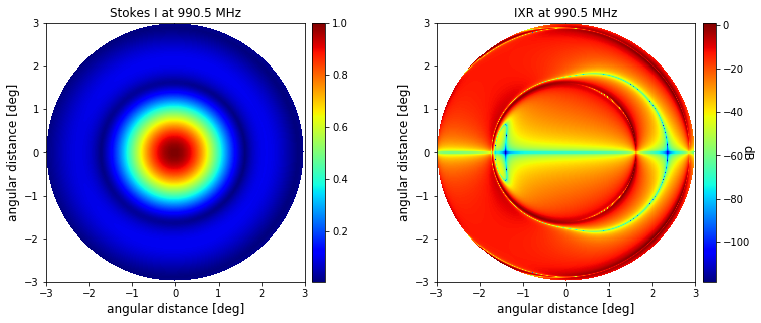
\includegraphics[scale=0.7]{c6/ixr/ixr990-5mhz}
%        \caption{bb}
%    \end{subfigure}
%    \end{figure}
%    
%    \begin{figure}
%\ContinuedFloat
%\centering
%    \begin{subfigure}{0.4\linewidth}
%        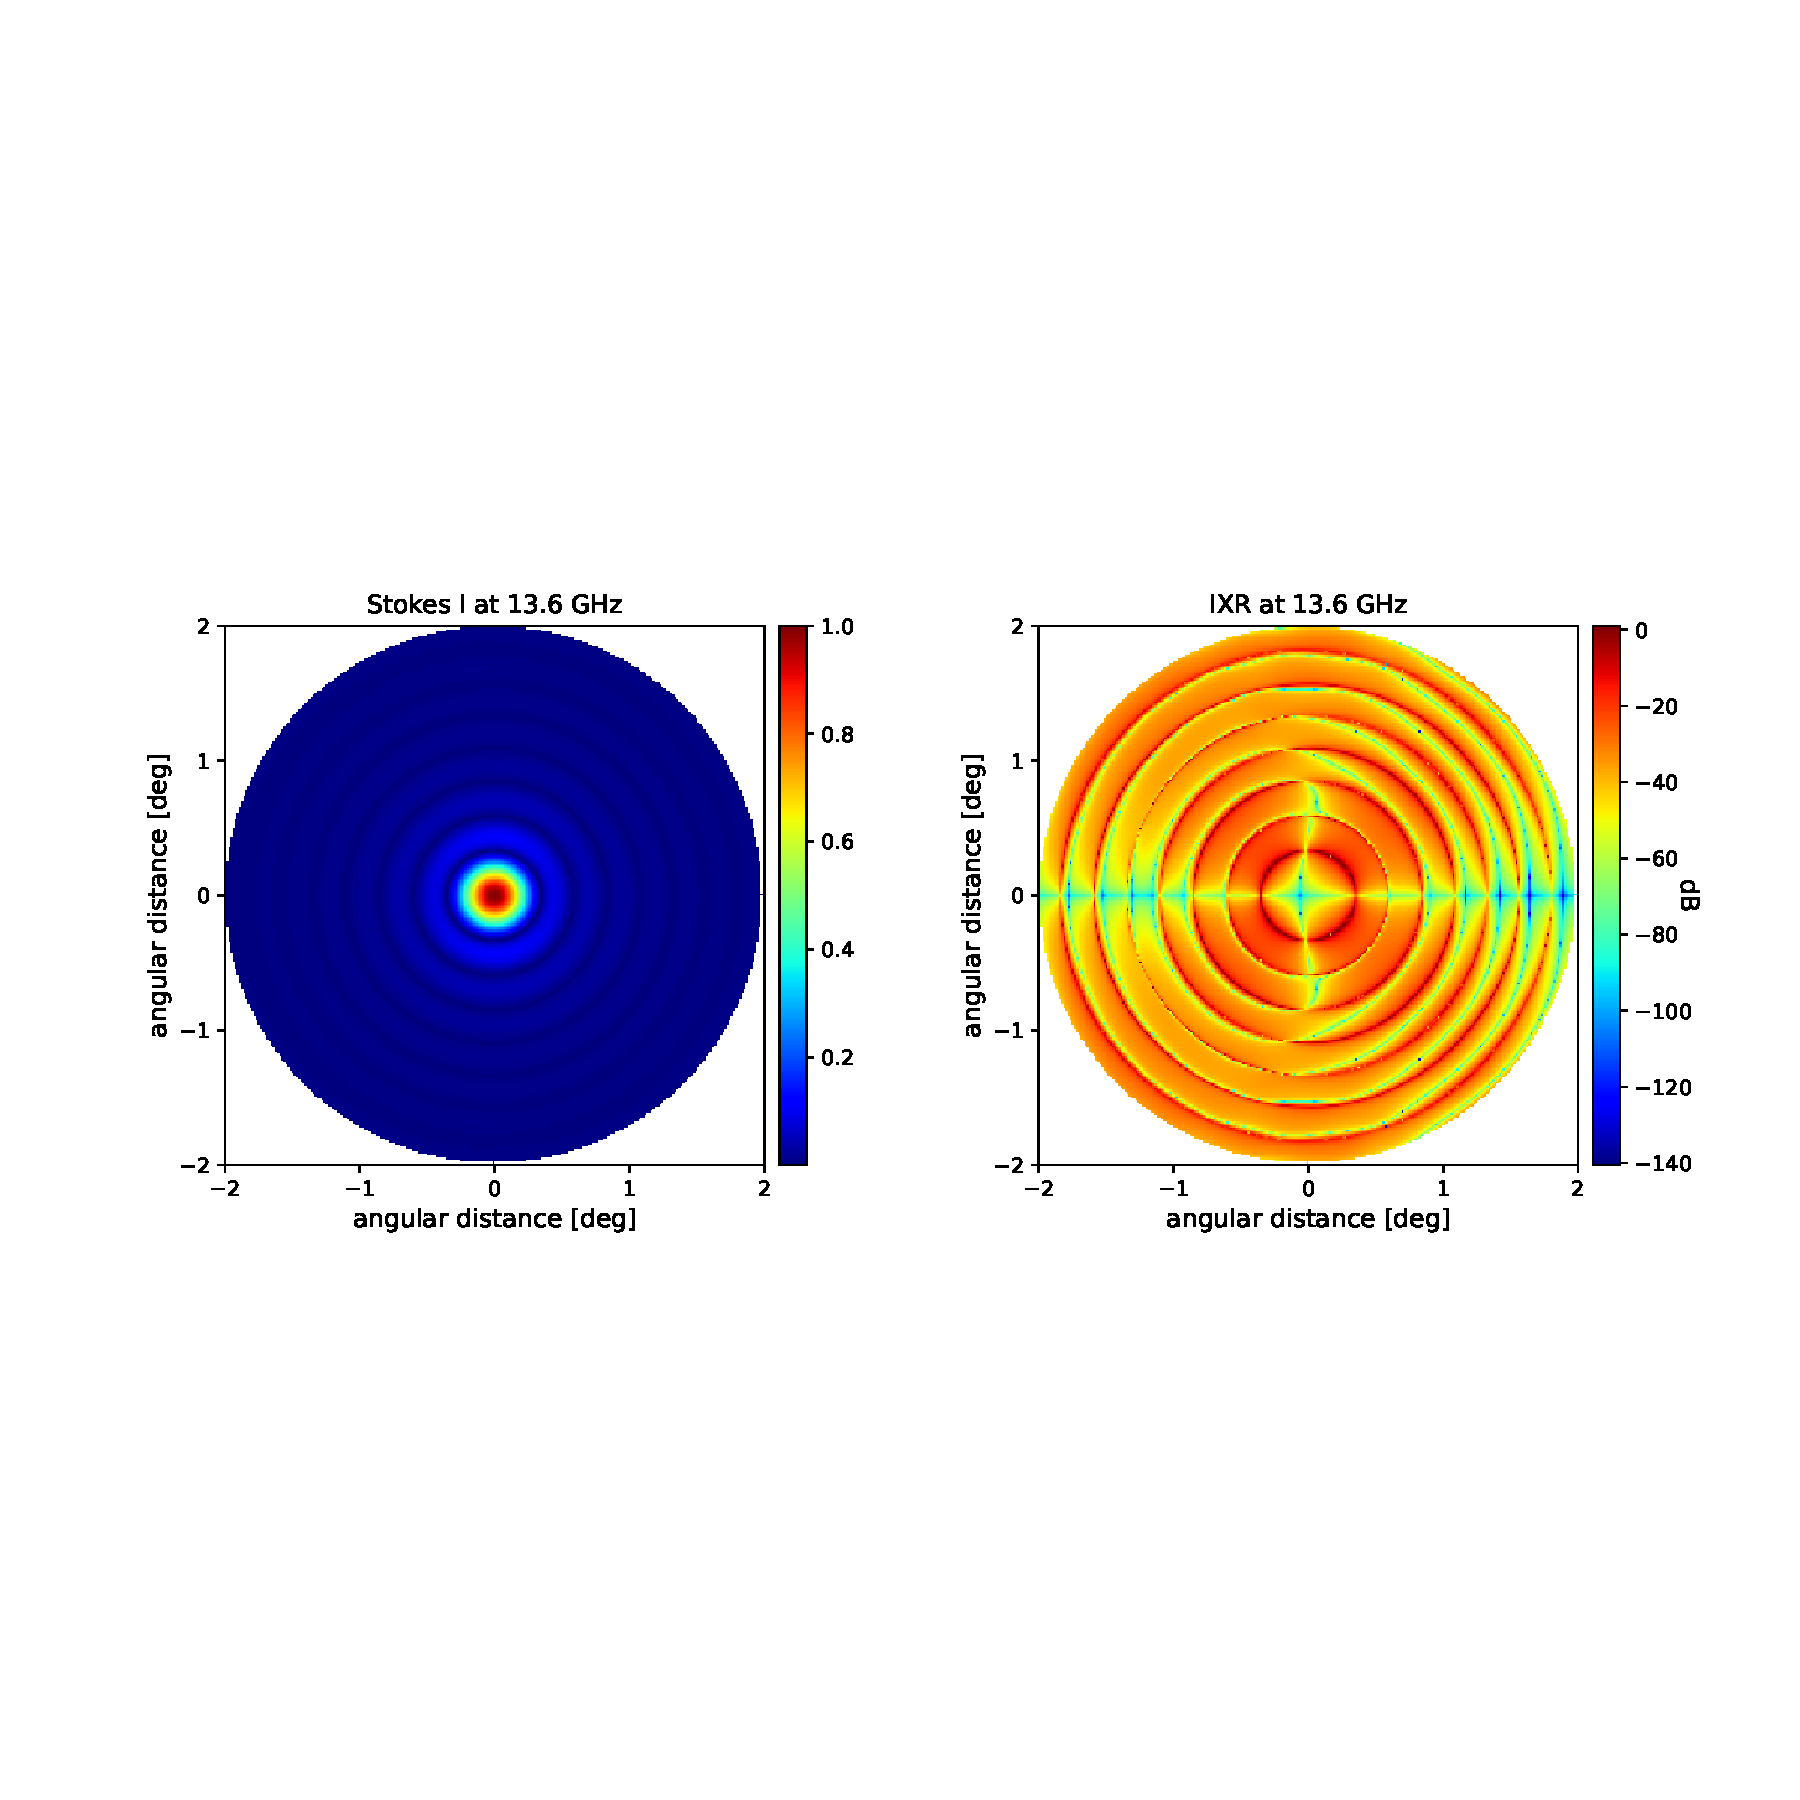
\includegraphics[scale=0.7]{c6/ixr/ixr_13-6}
%        \caption{tt}
%    \end{subfigure}
%    \caption{Several subfigures}
%\end{figure}
%
\begin{figure}[H]
%\begin{minipage}{\linewidth}
  \centering
     \begin{subfigure}[b]{1.0\textwidth}
                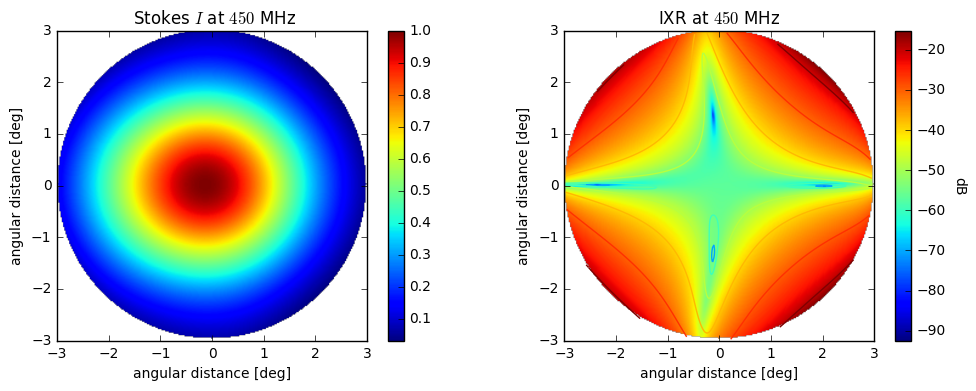
\includegraphics[width=\textwidth]{c6/ixr/ixr_450mhz}%ixr450} %zb1rad}
                \caption{}
                \label{fig:fg1a}
        \end{subfigure} \\
        \begin{subfigure}[b]{1.0\textwidth}
                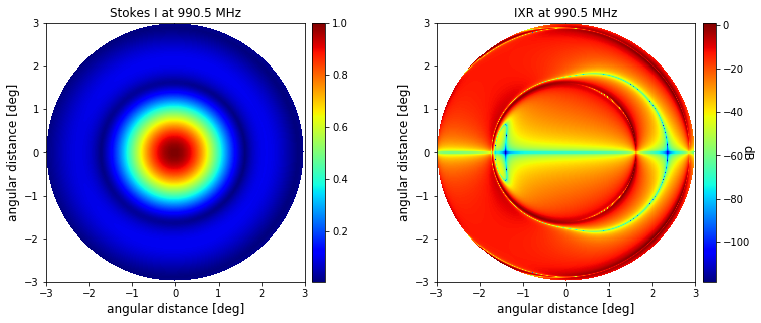
\includegraphics[width=\textwidth]{c6/ixr/ixr990-5mhz} %ixr13gh} %b5rad}
                \caption{}
               \label{fig:fg1b}
        \end{subfigure} \\
        \begin{subfigure}[b]{1.0\textwidth}
                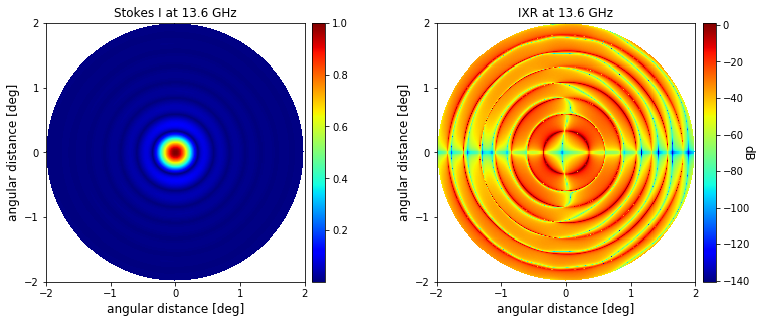
\includegraphics[width=\textwidth]{c6/ixr/ixr_13-6.png} %13ixr} %ixr_4-6ghz} %ixr4-6} %b5rad}
                \caption{}
               \label{fig:fg1c}
        \end{subfigure} 
%        \end{minipage}        
        \caption{Representation of $IXR_{\rm mu}$ (right panels) with the corresponding Stokes $I$ beams (left panels) at 450 MHz, 990.5 MHz and 13.6 GHz. Stokes I is computed in Jones terms as $(j_{\rm xx}j_{\rm xx}^{*}\, + j_{\rm xy}j_{\rm xy}^{*}\, + j_{\rm yx}j_{\rm yx}^{*}\, + j_{\rm yy}j_{\rm yy}^{*})/2$.}
    \label{fig:ixrbands}
  \end{figure} 
%%

\noindent Mathematically, we can present the IXR in Mueller form as:

\begin{equation}  \label{eq:ixr}
 IXR_{\rm mu} = 10\mathrm{log_{10}}\left( \frac{\sqrt{M_{IQ}^2 +M_{IU}^2 + M_{IV}^2}}{\lvert  M_{II}  \rvert} \right)
\end{equation}

\noindent The $IXR_{\rm mu}$ relates to the ideal rate of polarization leakage ($I$ into $QUV$ and in reverse) of the beam. Fig.~\ref{fig:ixrbands} shows the IXRs (the right plots) and the corresponding Stokes $I$ beams (the left plots) for the various bands. The expected IXR for SKA1-mid is maximized at $-20$ dB in the direction of the phase centre. Here, the negative dB units shown in the colour bar plots denote an increase in the seepage away from the observation phase centre. In addition, the rings in the IXR plots correspond to the beam nulls where the signals can not be detected. Note how the ring spacing scales with frequency. 

Now that we are well-informed about the SKA1-mid primary beams, we apply these with the foreground simulation discussed in Chapter~\ref{Chapter3} to estimate the spectral lines
in this chapter. Next, we discuss the CO spectrum at $z\sim3$.

%  \section{Modelling CO Emission}
%  %%
%  
%  In this section we will outline our method for modelling the power spectrum of CO fluctuations. In order to understand the derivation of CO temperature refer
%  to \citet{Breysse:2014uia}. Here, we concentrate on the methods to adopt to estimate the angular spectrum distribution of CO emission.
%  
 
 
 \section{The CO Power Spectrum}
 
 \enquote{In order to derive the power spectrum to be observed in typical CO intensity mapping experiments, one also needs to model the clustering of the CO sources. In analogy with the methods for other species, e.g., neutral hydrogen intensity mapping, this can be done by weighting the dark matter halo bias by the CO luminosity-halo mass relation}  \citep{2018MNRAS.475.1477P}.

 
%  With the view to estimate the angular power spectrum of CO emission ($C_l$) , we have to deduce the underlying 3D mass distribution to $C_l$.
%  The brief description below shows the approach of \citet{Huterer:2000uj,Tegmark:2001xb,Blake:2004dg,Padmanabhan:2006cia,Thomas:2010wi}.  
%  The angular power spectrum $C_l$ is a projection  of the spatial power spectrum of mass fluctuations at different red-shifts,  $P(k, z)$, where $k$ is a co-moving wavenumber. In linear perturbation theory, fluctuations with different
% $k$ evolve independently, scaling with redshift according to the growth factor $D(z)$. Under this assumption we can simply scale the 
% present-day matter power spectrum $P_{0}(k)$ back with redshift:
% %%
Here, the intensity of the CO signal $S_{\rm P}^{\rm CO}$ is expressed as a wavenumber $k_{w}$ at every $z$:
\begin{equation}  \label{eq:ps1}
S_{\rm P}^{\rm CO}(k_{w},z) = \langle T_{\rm b}^{\rm CO} \rangle (z)^{2}[d_{\rm b}^{\rm CO}(z)^{2} S_{\rm lin}(k_{w},z) + S_{\rm shot}(z)] 
\end{equation}

\noindent where $T_{\rm b}^{\rm CO}$ is the CO brightness temperature, $d_{\rm b}^{\rm CO}$ is the CO halo bias source, $S_{\rm lin}$ is the power spectrum of linear matter,
and $S_{\rm shot}$ is the addition of shot noise to the power spectrum.

Modelling the system in Equation~\ref{eq:ps1} as a linear relation and projecting the CO intensity distribution into spherical form, we obtain a reduce function 
over the halo mass as given in Equation~\ref{eq:ps2}:

\begin{equation}  \label{eq:ps2}
 C_{l} = \langle T_{\rm b}^{\rm CO} \rangle (z)^{2}\int S_{\rm lin}(k_{w},z)W_{l}(k_{w}) dk_{w}
\end{equation}

\noindent  The kernel function $W_{l}(k_{w})$ in Equation~\ref{eq:ps2} is defined in spherical Bessel expression as:
%%
\begin{equation}  \label{eq:ps3}
 W_{l}(k_{w}) = \frac{2}{\pi}\left[ \int_{0}^{\infty}  j_{l}(u) f(u/k_{w}) du \right]^2
\end{equation}

\noindent  where  $f(u/k_{w})$ is the weight describing the  distribution of the source. 
%%
% \begin{equation}  \label{eq:ps4}
%  f_{z}(x) = p(z)D(z)b(z)\frac{dz}{dx}
% \end{equation}
% 
% \noindent  In Equation~\ref{eq:ps4}, $x$ is the co-moving radial coordinate at redshift $z$, $p(z)$ is the redshift probability distribution of the sources, such that
% the normalised form is defined as $\int p(z) dz = 1$ and the linear bias factor $b(z)$  correlates the clustering of galaxies to clustering of the underlying mass such that
% $P_{gal}(k,z) = b(z)^{2}P_{mass}(k,z) $.


\noindent At large $l$, we can approximate the spherical Bessel function in Equation~\ref{eq:ps3} such that $j_{l}(x) \approx \sqrt{\frac{\pi}{2l}} \delta(x-l)$ to get:
\begin{equation}  \label{eq:ps5}
 W_{l}(k) \approx \frac{1}{l} f(l/k_{w})^2
\end{equation}

\noindent  Therefore, as $l$ becomes large, the kernel function changes along the $k_{w}$-axis. Replace  Equation ~\ref{eq:ps5} into~\ref{eq:ps2} obtain the angular spectrum:
\begin{equation}  \label{eq:ps6}
 C_{l} \approx \langle T_{\rm b}^{\rm CO} \rangle (z)^{2}\frac{1}{l} \int S_{\rm lin}(k_{w},z)f(l/k_{w})^2 dk_{w}
\end{equation}


\noindent  Therefore, at $z \sim 3$, the signal is expected to be at most $1.5\, \mathrm{\mu K}$ at the halo bias level of $b(z) = 0.2$ \citep{2011ApJ...728L..46G}. Using this
normalisation constant, we can translate Equation~\ref{eq:ps6} into an integral over radial co-ordinate:


\begin{equation}  \label{eq:ps7}
  C_{l} \approx 2.25\times 10^{-06}\int S_{\rm lin}(k_{w},z)f(l/k_{w})^2 dk_{w} \quad [\mathrm{mK^2}]
\end{equation}

\noindent  Due to the variations in gravitational energy and mass density, we consider the spatial spectrum to have a power law such that
$S_{\rm lin}(k_{w},z) \alpha k_{w}^n$ and therefore, we can evaluate the angular spectrum as $C_{l} \alpha l^n$.
For $n = 1$ gives $C_{l}  \alpha \frac{1}{l(l+1)}$ at low $l$. 
%%

In this work, we adopt the {\tt CAMB}\footnote{\url{ http://camb.readthedocs.io/en/latest/}} software package to compute the $C_{l}$ of CO signal at $z=3$.
This package is able to set cosmological parameters in terms of physical densities and parameters used in \cite{Ade:2015xua}. %Planck 2015 analysis 
% pars.set_cosmology

%  def set_cosmology(self, H0=67, ombh2=0.022, omch2=0.12, omk=0.0, num_massive_neutrinos=1, mnu=0.06, nnu=3.046,
%                       YHe=None, meffsterile=0, standard_neutrino_neff=3.046, TCMB=constants.COBE_CMBTemp, tau=None,
%                       tau_neutron=bbn.tau_n):
%         """
%         Sets cosmological parameters in terms of physical densities and parameters used in Planck 2015 analysis.
%         Assumes a single distinct neutrino mass eigenstate, by default one neutrino with mnu = 0.06eV.
%         If you require more fine-grained control can set the neutrino parameters directly rather than using this function.
% 
%         :param H0: Hubble parameter (in km/s/Mpc)
%         :param ombh2: physical density in baryons
%         :param omch2:  physical density in cold dark matter
%         :param omk: Omega_K curvature parameter
%         :param num_massive_neutrinos:  number of massive neutrinos
%         :param mnu: sum of neutrino masses (in eV)
%         :param nnu: N_eff, effective relativistic degrees of freedom
%         :param YHe: Helium mass fraction. If None, set from BBN consistency.
%         :param meffsterile: effective mass of sterile neutrinos
%         :param standard_neutrino_neff:  default value for N_eff in standard cosmology (non-integer to allow for partial
%                 heating of neutrinos at electron-positron annihilation and QED effects)
%         :param TCMB: CMB temperature (in Kelvin)
%         :param tau: optical depth; if None, current Reion settings are not changed
%         :param tau_neutron: neutron lifetime, for setting YHe using BBN consistency
%         """
\section{Results and Analysis} 
%%

Repeating the full-sky simulation discussed in Chapter~\ref{Chapter4}, we perform IM experiments by convolving the foregrounds in 
Figs.~\ref{fig:f450},~\ref{fig:f990}, and ~\ref{fig:f1306} with the simulated {\tt GRASP} beams (original EM beams), Zernike reconstructed beams and the distorted modelled beams 
for each band (at 450 MHz, 990.5 MHz and 13.6 GHz). Note here that these voltage beams must first be converted into  their Mueller forms before applying them to the polarized sky maps.
Fig.~\ref{fig:erD1} shows the systematic error maps\footnote{{\tt The grey parts of the error plots are masked galaxies.}} for Band $1$ (at 450 MHz) when we compute
the differences between the convolved foregrounds using the fully polarized {\tt GRASP} beams (in Mueller form) that are obtained from the beams in Fig.~\ref{fig:band1} (Data row) 
and the distorted beams in Fig.~\ref{fig:bandD1} (Distorted row). Fig~\ref{fig:erZ1} also shows the the differences between the measured foregrounds using the same {\tt GRASP} beams in Fig.~\ref{fig:band1} (Data row) and Zernike beams in Fig.~\ref{fig:band1} (Model row). 
Similar explanations can be given to the error maps in Figs.~\ref{fig:erD2},~\ref{fig:erZ2} and Figs.~\ref{fig:erD},~\ref{fig:erZ} for using Bands $2$ (at 990.5 MHz) and $5$ (at 13.6 GHz) fully polarized primary beams accordingly.

\begin{figure}
\begin{minipage}[H]{\linewidth}
\centering
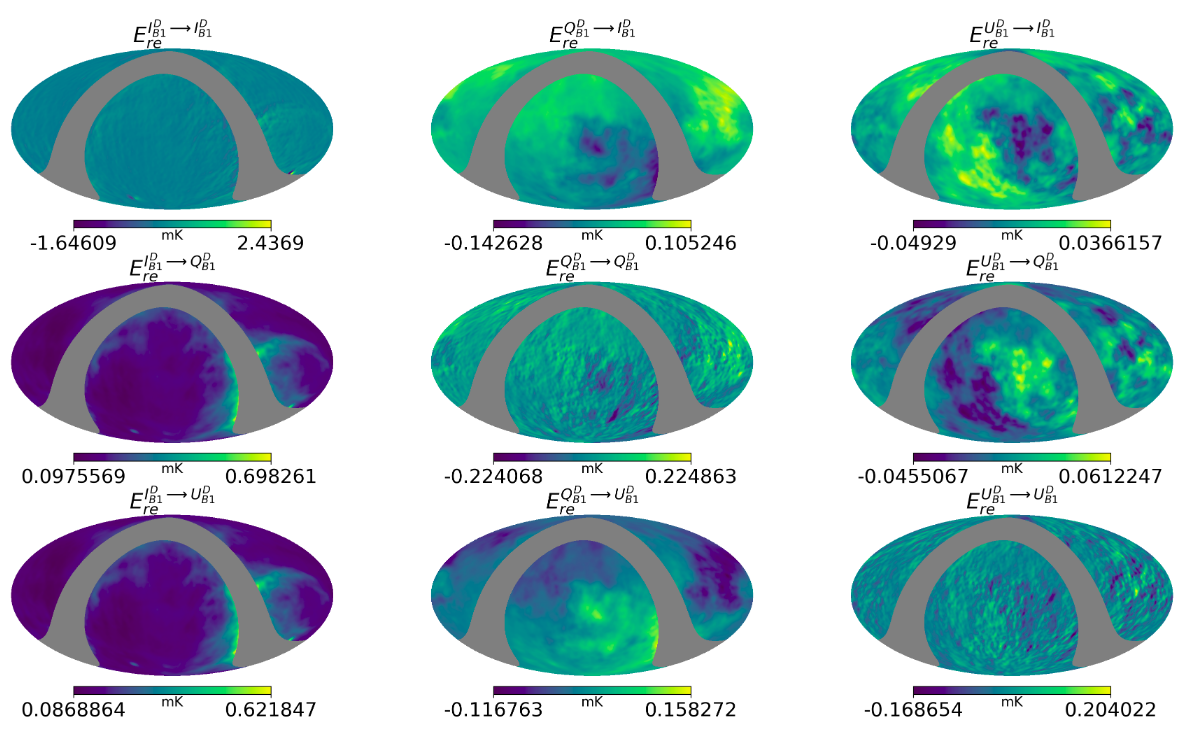
\includegraphics[width=1.2\linewidth]{/c6/grasp/b1D} %band_1_errD1}
\caption{\label{fig:erD1} Systematic errors of the measured maps in Stokes I, Q, U, due to feed displacement at $450$ MHz.
}
\end{minipage}
\end{figure}
\FloatBarrier

\begin{figure}
\begin{minipage}[H]{\linewidth}
\centering
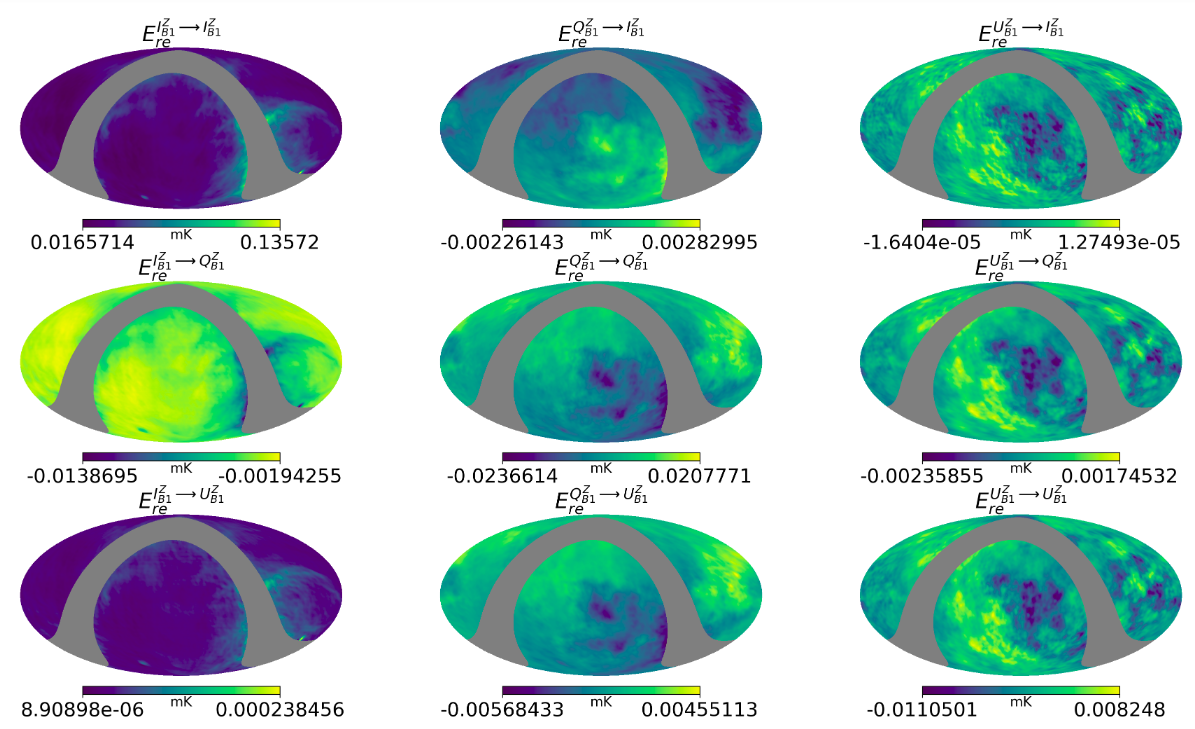
\includegraphics[width=1.2\linewidth]{/c6/grasp/b1Z} %band_1_errZ}
\caption{\label{fig:erZ1} Systematic errors of measured maps using Zernike model beams at $450$ MHz.}
\end{minipage}
\end{figure}
\FloatBarrier


\begin{figure}
\begin{minipage}[H]{\linewidth}
\centering
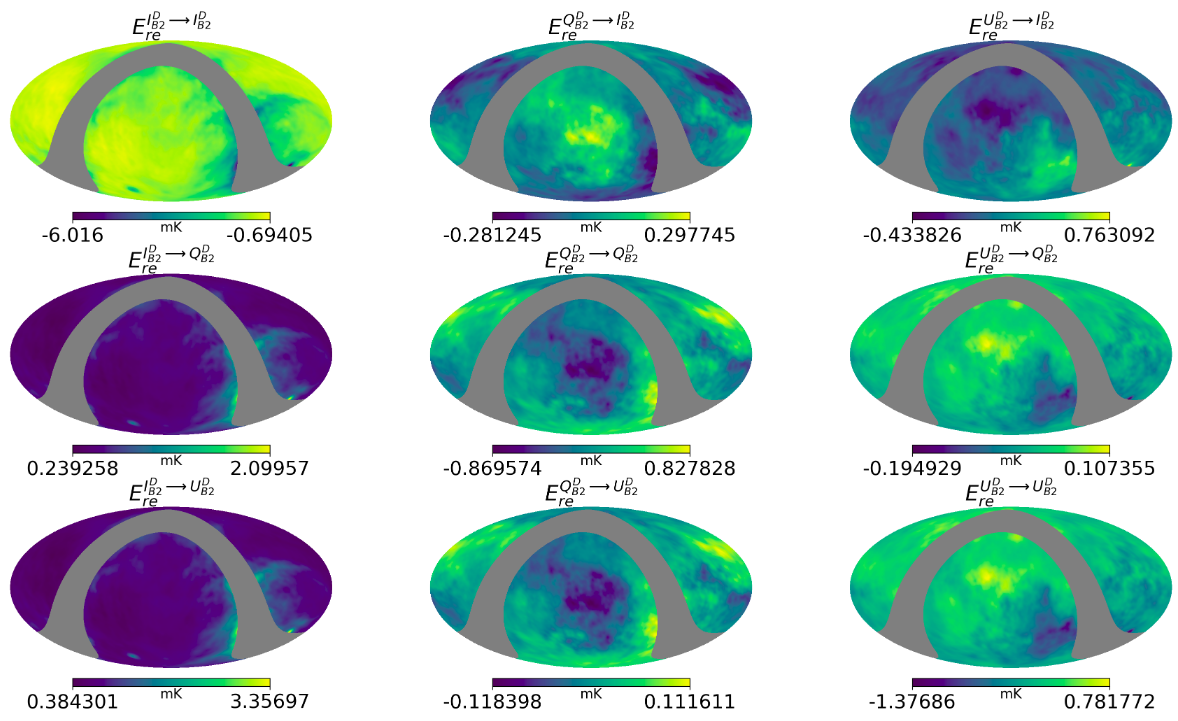
\includegraphics[width=1.2\linewidth]{/c6/grasp/b2D} %band_2_errD}
\caption{\label{fig:erD2} Systematic errors of measured maps due to feed displacement at $990.5$ MHz.}
\end{minipage}
\end{figure}
\FloatBarrier

\begin{figure}
\begin{minipage}[H]{\linewidth}
\centering
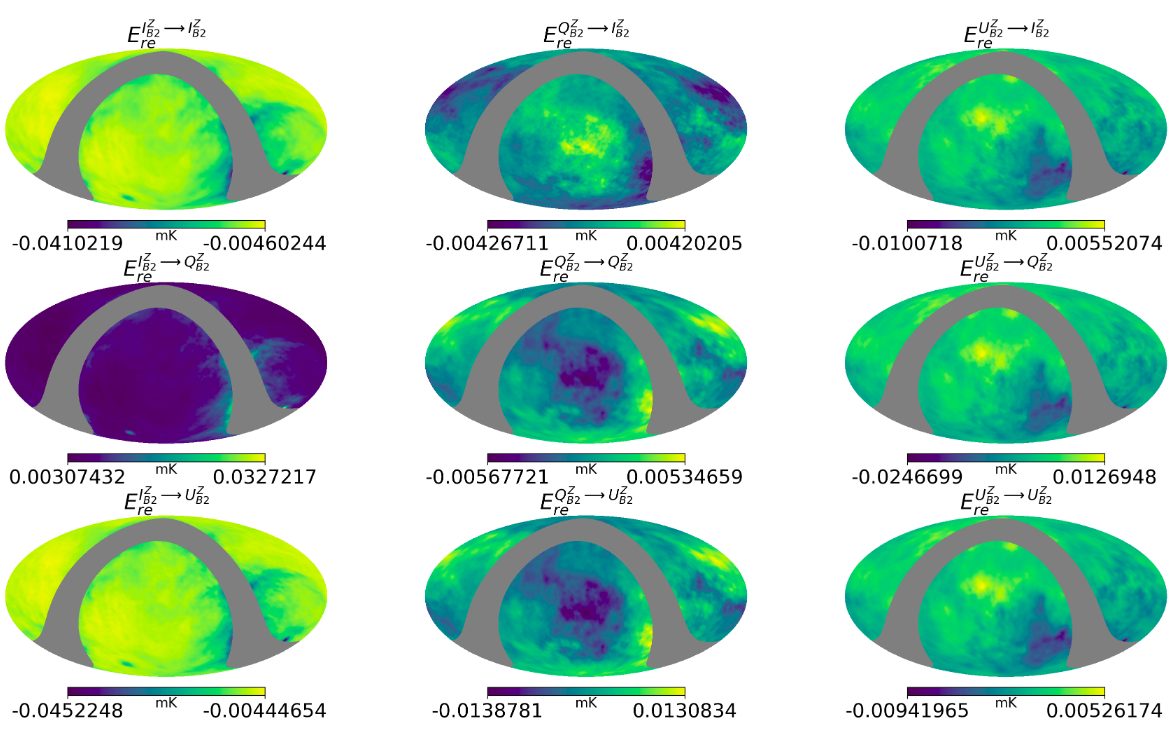
\includegraphics[width=1.2\linewidth]{/c6/grasp/b2Z} %band_2_errZ}
\caption{\label{fig:erZ2} Systematic errors of measured maps using Zernike model beams at $990.5$ MHz.}
\end{minipage}
\end{figure}
\FloatBarrier

% B 5

\begin{figure}
\begin{minipage}[H]{\linewidth}
\centering
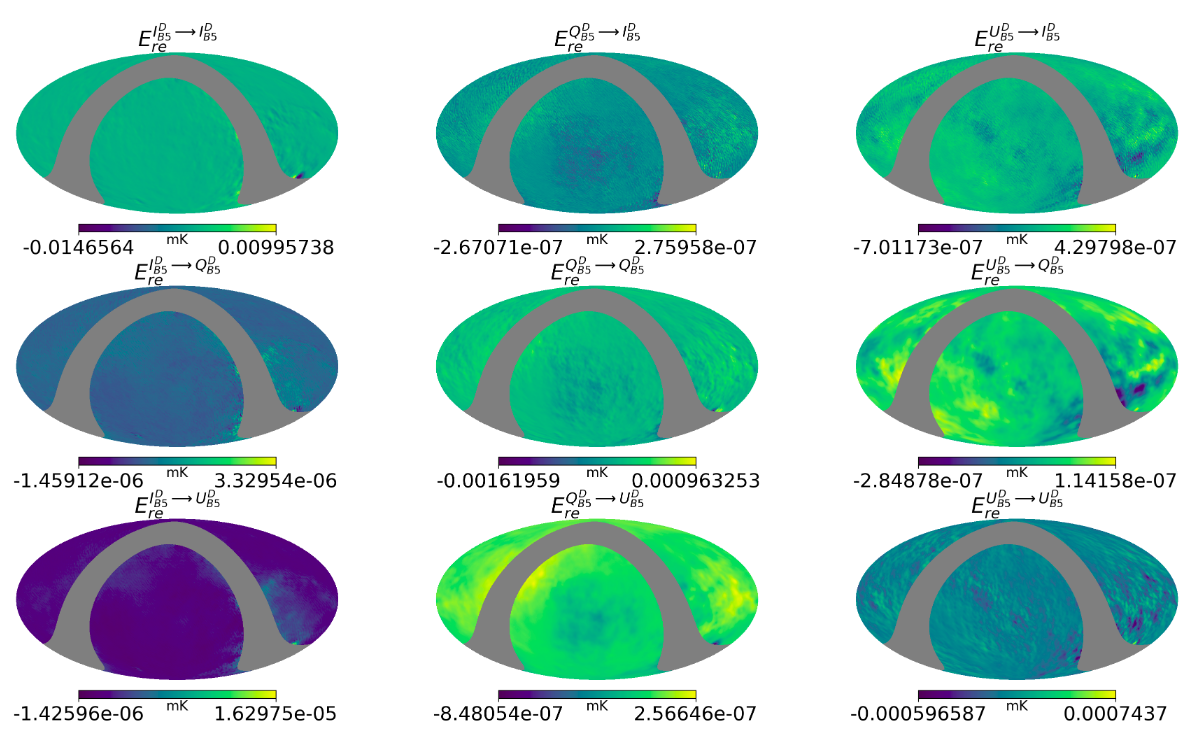
\includegraphics[width=1.2\linewidth]{/c6/grasp/b5D} %band_5_errD}
\caption{\label{fig:erD} Systematic errors of measured maps due to feed displacement at $13.6$ GHz.}
\end{minipage}
\end{figure}
\FloatBarrier

\begin{figure}
\begin{minipage}[H]{\linewidth}
\centering
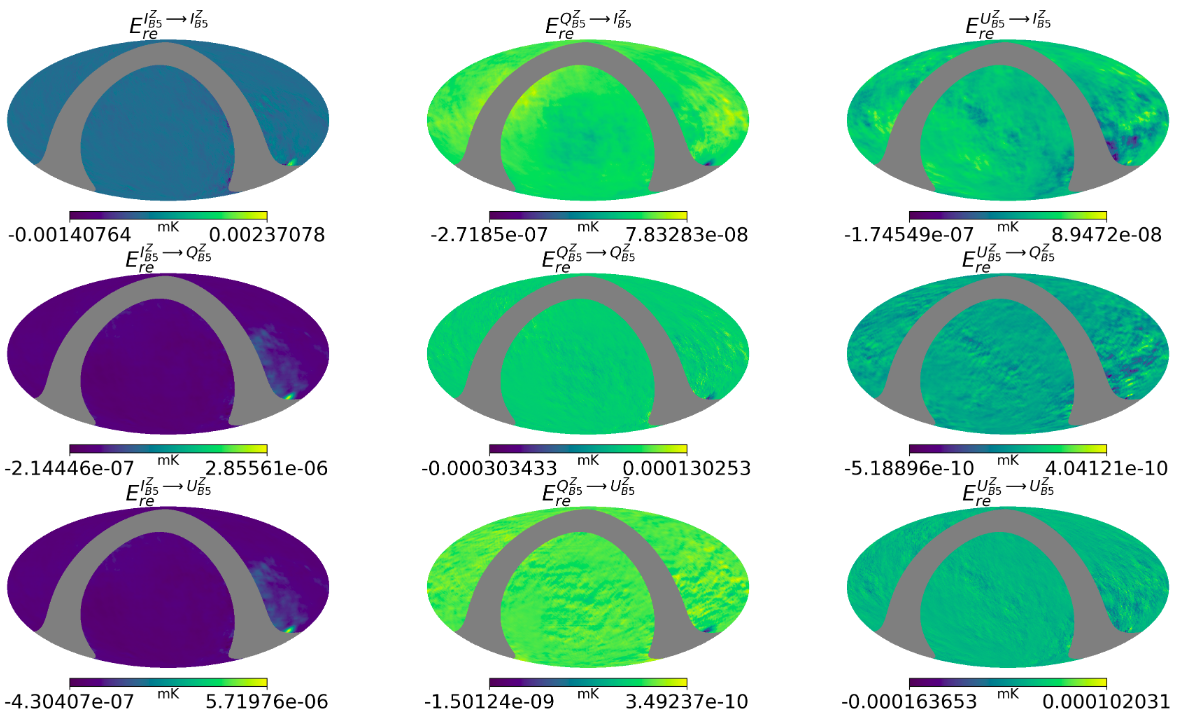
\includegraphics[width=1.2\linewidth]{/c6/grasp/b5Z} %band_5_errZ}
\caption{\label{fig:erZ} Systematic errors of measured maps using Zernike model beams at $13.6$ GHz.}
\end{minipage}
\end{figure}
\FloatBarrier
%%

% shows the measured Stokes and the corresponding errors in Stokes $I, Q$ and $U$ 

\noindent Fig.~\ref{fig:b5ALL} is produced when we convolve the full-sky polarization maps in Fig.~\ref{fig:f1306} with the primary beams at 13.6 GHz. 
The maps in the first row are the convolved foregrounds, using the complete beams of the original simulated {\tt GRASP} model in Fig.~\ref{fig:band5a} (Data row). 
The second row is obtained for using the perturbed beams in Fig.~\ref{fig:bandD5a} (Distorted row) and the third row is as a result of using the Zernike beam models 
in Fig.~\ref{fig:band5a} (Model row). The remaining two rows are the respective errors in Stokes $I, Q$ and $U$ for using distorted
and reconstructed beam models. Next, we quantify the foregrounds measured by transforming these spatial distributions into spherical harmonics to determine the angular power
spectrum.

%%

\begin{figure}
\begin{minipage}[H]{\linewidth}
\centering
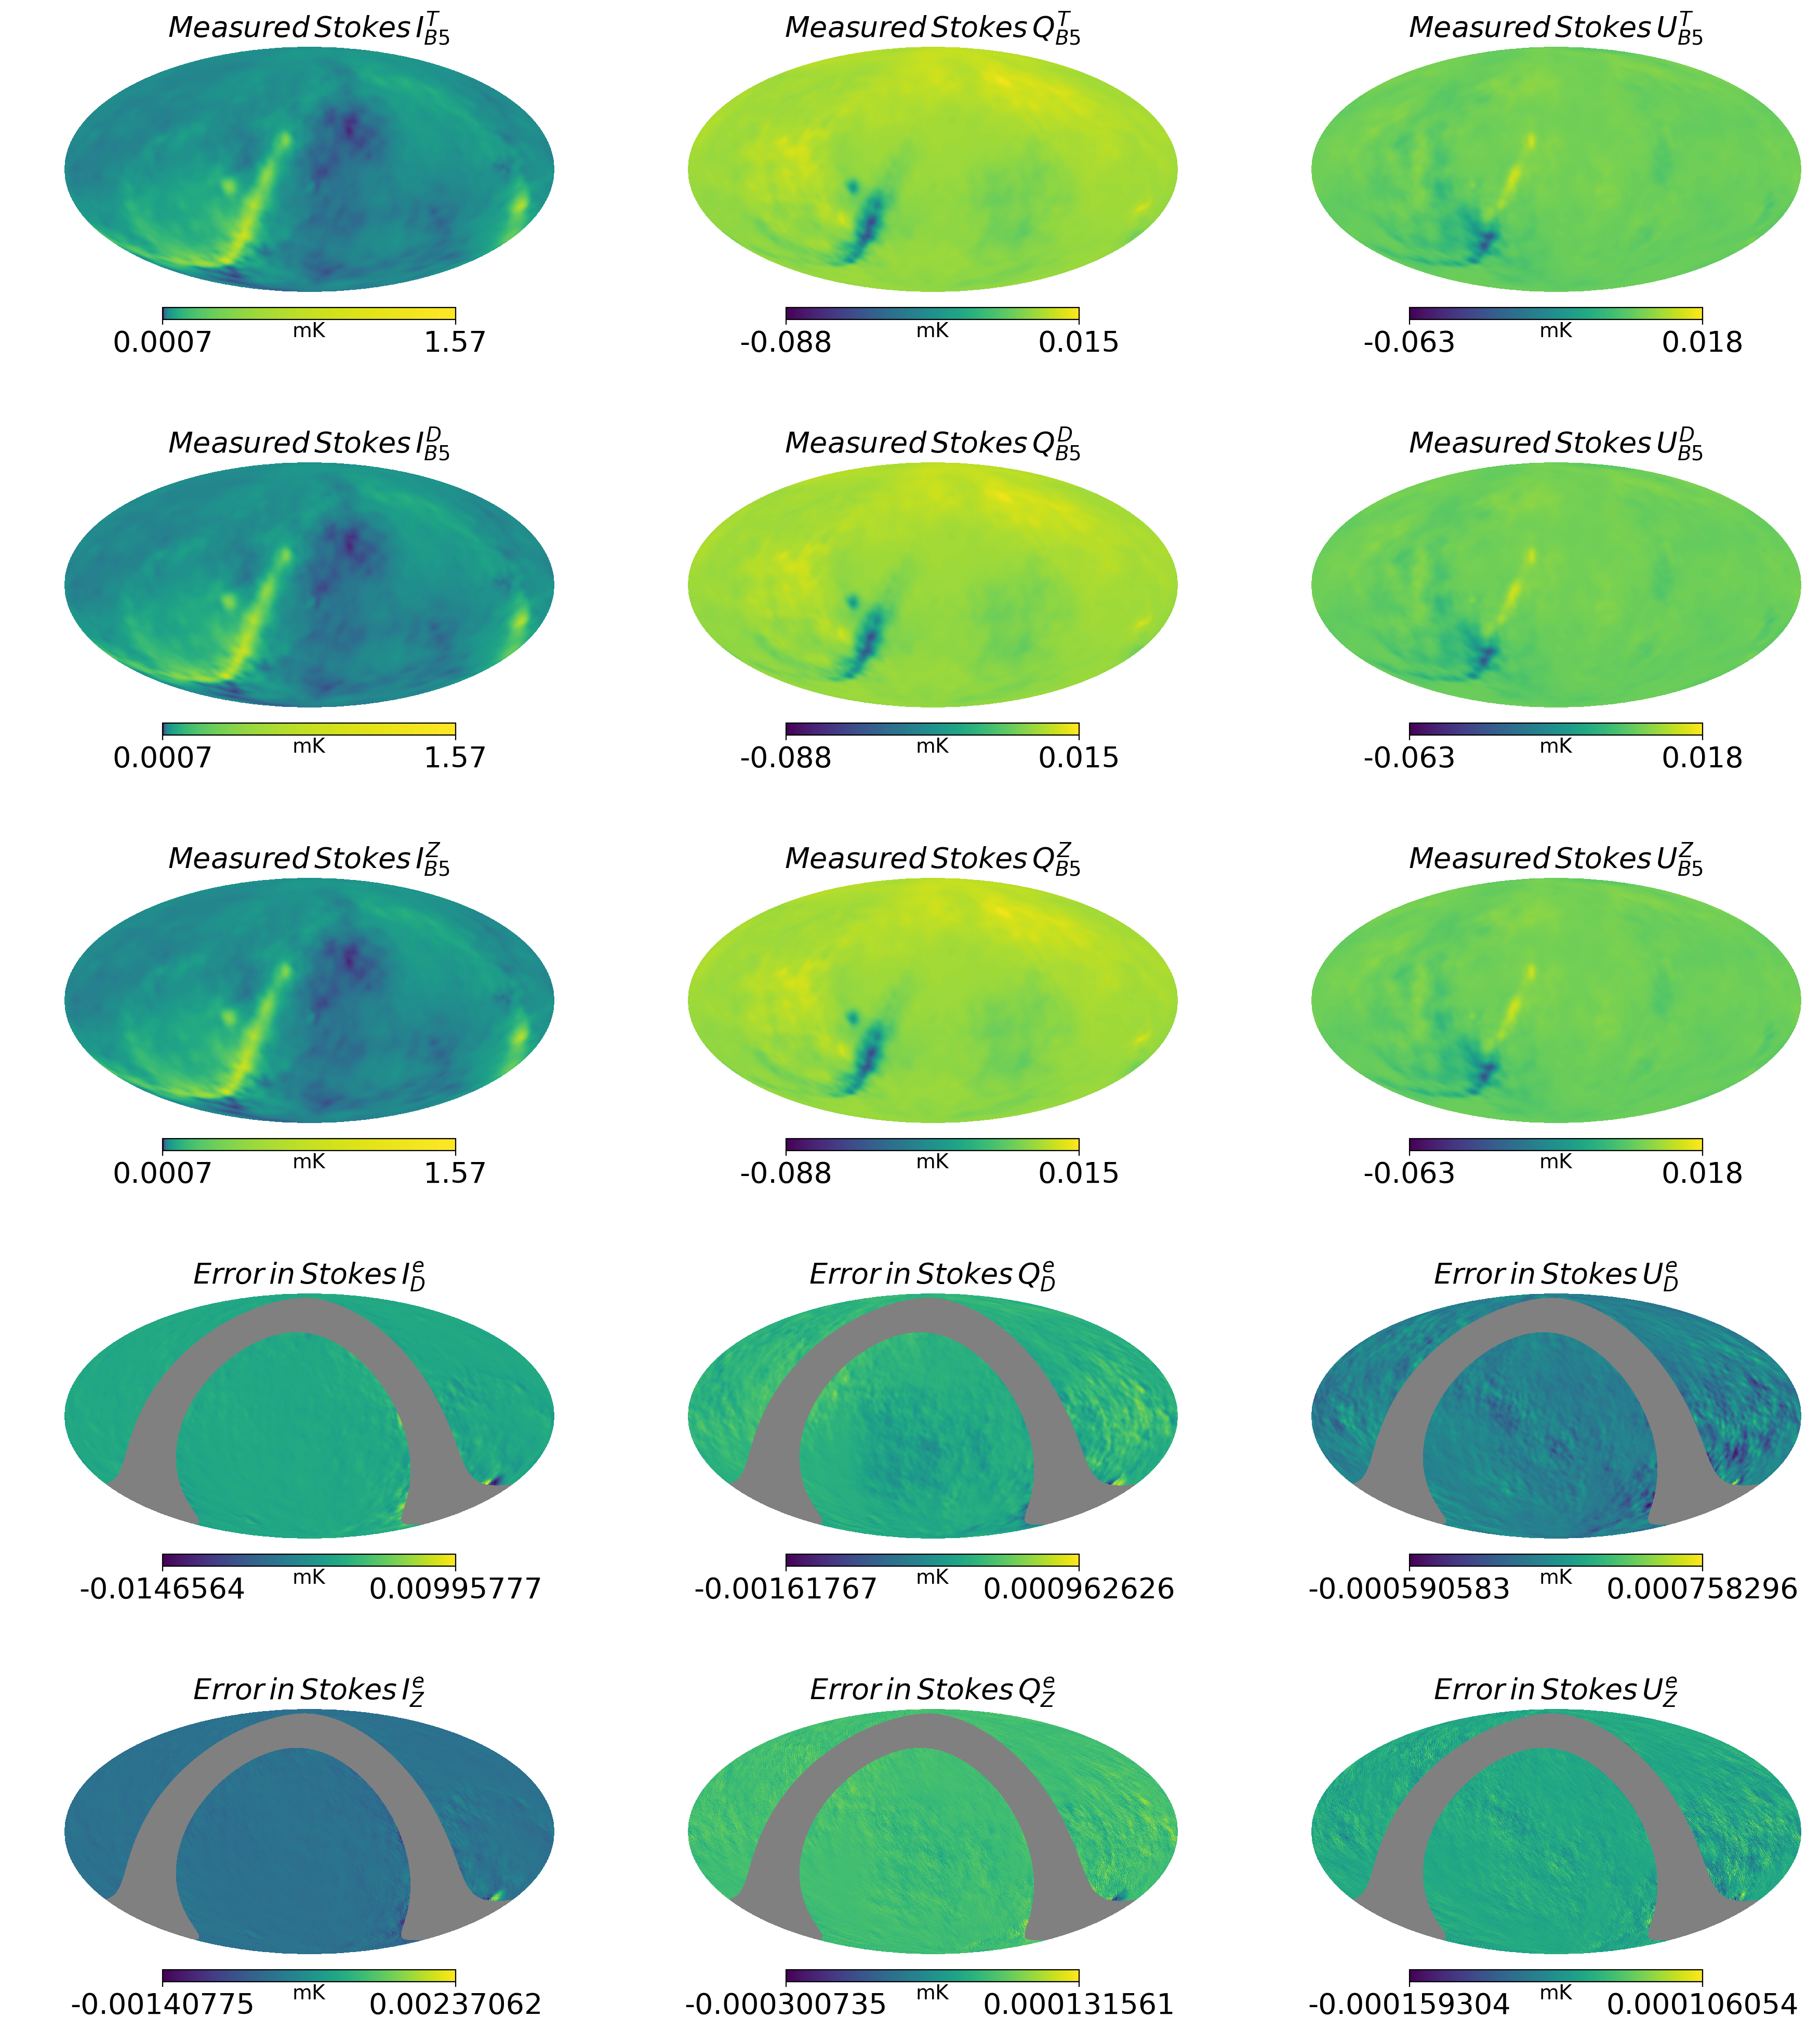
\includegraphics[width=1.2\linewidth]{/c6/grasp/B5zCV} %band_5_ALL}
\caption{\label{fig:b5ALL} Convolved full-sky maps at $13.6$ GHz  with respective error in Stokes $I, Q$ and $U$.}
\end{minipage}
\end{figure}
\FloatBarrier
% 

The power spectra plots reported in Fig.~\ref{fig:HC} enable us to estimate both the HI (grey-magenta circular spectral plots) and CO (grey spectral plots) signals at a specific
multipole moment. The left spectra plots in Figs.~\ref{fig:H1},~\ref{fig:H2},~\ref{fig:Co} show how we recovered the HI and CO signals in Stokes $I$ when the errors 
in the primary beams of a particular band are corrected. For instance, in Band $1$ (at 450 MHz), when the beam errors are corrected in Stokes $I$, we expect 
the HI signal at $z \approx 0.67$ to be measured at a multipole moment of $l \lesssim 50$ which is about $3$ orders of magnitude greater than that of the foreground at lower scales. 
In the case of Band $2$ (at 990.5 MHz), the HI signal is also measured at a multipole moment of $l \lesssim 50$ and about $4$ orders of magnitude greater than the foreground at lower scales. For the Band $5$ (at 13.6 GHz),
the CO signal at $z \approx 3$ is expected to be measured at a multipole moment of $l \ll 50$ which is about $3$ orders of magnitude lower than the foreground at lower scales. 
On the other hand, the right spectra plots in Figs.~\ref{fig:H1},~\ref{fig:H2},~\ref{fig:Co} show how we measure the signals when the intrinsic linear polarization leakage in Stokes $I$ is known
whilst the  errors in the primary beams of a particular band are not corrected. The power spectrum of the HI signal for Bands $1$ and $2$ can be estimated at a 
multipole moment of $\approx 50$ and $\approx 100$ respectively. For Band $5$, the estimated power spectrum of the CO signal can be estimated up to
a multipole moment of $\approx 50$. In addition, the spectra plots due to Zernike model of the beam for all bands clearly predicted both the HI and CO signals to be 
at a multipole moment of $l \lesssim 50$, making Zernike fitting a good  reconstructed model for intensity mapping experiments.

\begin{figure}[H]
  \centering
     \begin{subfigure}{\columnwidth}
                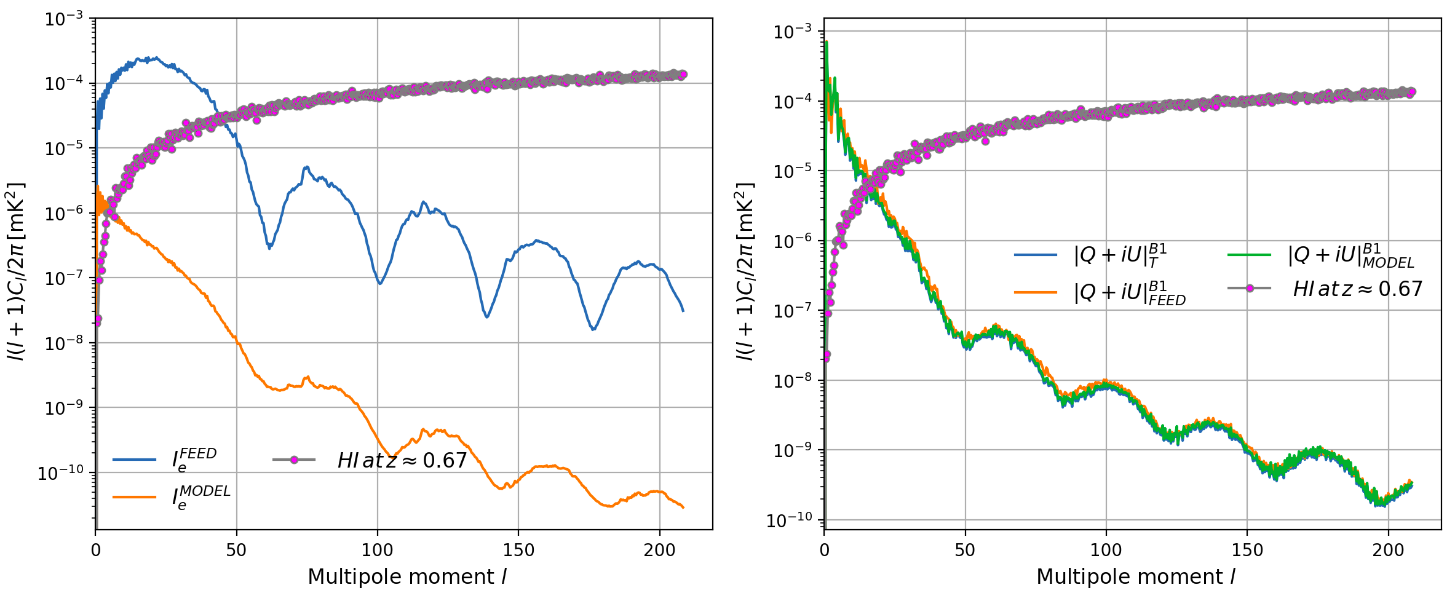
\includegraphics[width=\linewidth]{/c6/hb1a} %grasp/band_1_HIsim}
                \caption{}
                \label{fig:H1}
        \end{subfigure} \hfill
        %%
        \begin{subfigure}{\columnwidth}
                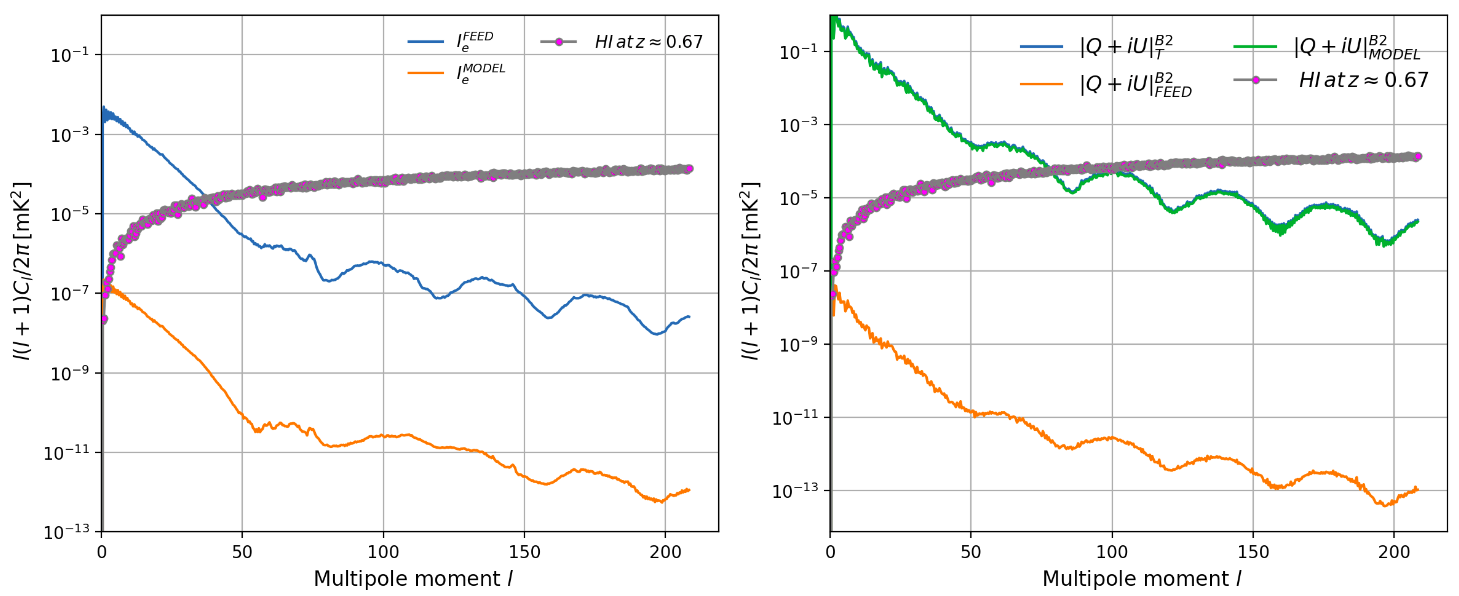
\includegraphics[width=\linewidth]{/c6/hb2} %band_2_HIsim}
                \caption{}
               \label{fig:H2}
        \end{subfigure} \hfill
        %%
        \begin{subfigure}{\columnwidth}
                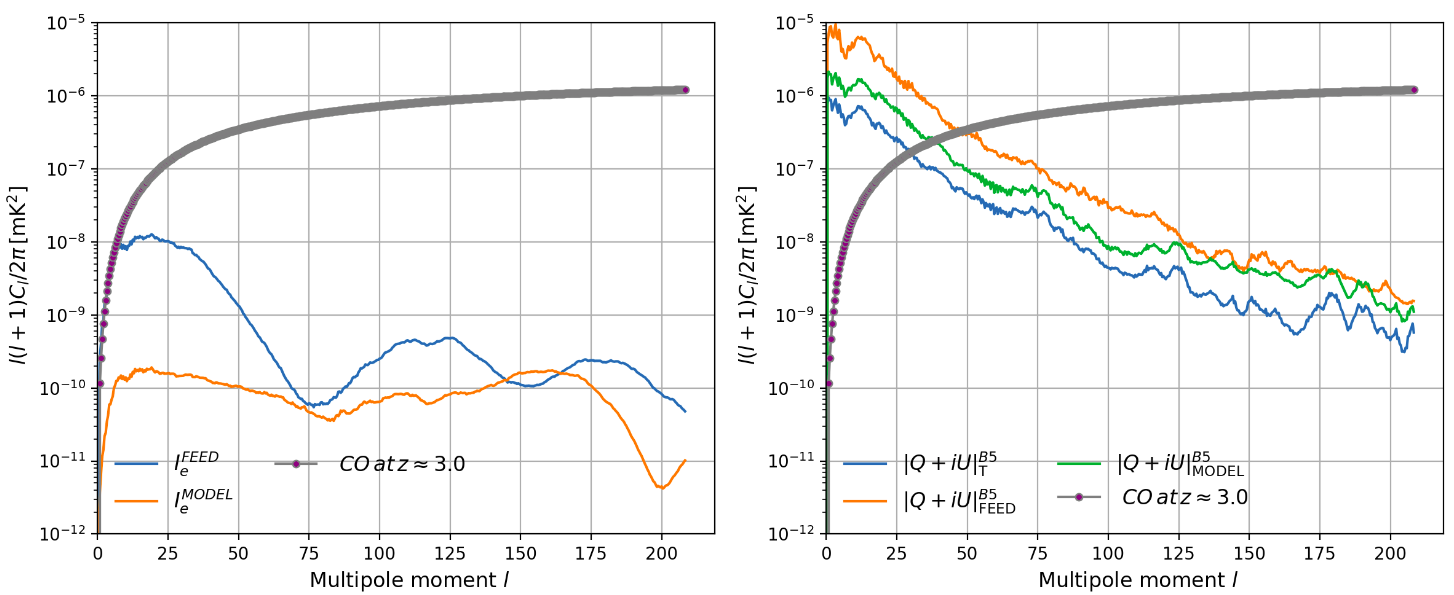
\includegraphics[width=\linewidth]{/c6/hb5b} %index}
                %{/c6/grasp/band_5_HIsim}
                \caption{}
               \label{fig:Co}
        \end{subfigure}
        
        \caption{Comparing the distribution of angular power plots between corrected beam errors due to Zernike fits or feed displacement
        in Stokes $I$ map (left plots) and  intrinsic polarization leakage in $I$ (right plots) and how these affect both the $21$ 
        cm and CO signal (solid circular spectrum plot). (a) For Band $1$ at $450$ MHz  (b) For Band $2$ at $990.5$ MHz  (c) For Band $5$ at $13.6$ GHz 
      }
	    \label{fig:HC}
  \end{figure}


%         """
\section{Conclusion} 
%%


This work showed how to simulate EM primary beams of SKA1-mid for Bands $1,2$ and $5$ using {\tt GRASP}, a commercial software package. A Zernike fit was then
used to reproduce these EM beams and then went on further to produce errors beams by including a systematic phase perturbations across the aperture 
to corrupt the beam pattern. HI IM experiment was performed with the primary beams of Bands $1$ (at 450 MHz) and $2$ (at 990.5 MHz) and then CO IM with Band $5$ (at 13.6 GHz) 
in order to estimate the power spectrum of both HI and CO signals. The following are the key findings of the research:
%%
\begin{itemize}
 \item We can use the MSE approach to choose the required number of Zernike modes with the corresponding coefficients to reconstruct the beams. Here,
       we select the modes where the MSE converges (refer to Fig.~\ref{fig:nmodes}). Note that the selected coefficients are what we define as the strongest coefficients.
      
%  The co- and cross-polarization level of amplitude ($\rho$) for Band $1$ (refer to Fig.~\ref{fig:cutsB1}) at different spherical cuts are within the 
%   range of ($-20 \leqslant \rho \leqslant 40$) dB and ($-40 \leqslant \rho \leqslant 10$) dB respectively, that of Band $2$ (refer to Fig.~\ref{fig:cutsB2})
%   are ($-10 \leqslant \rho \leqslant 40$) dB and ($-40 \leqslant \rho \leqslant 10$) dB respectively and then for 
%   Band $5$ (refer to Fig.~\ref{fig:cutsB5}) we have ($0 \leqslant \rho \leqslant 60$) dB and ($-20 \leqslant \rho \leqslant 30$) dB respectively.
  \item Reconstructing the original EM beams with the Zernike model, produces a maximum residual error of 
  $\simeq 1 \%$ (refer to the bottom rows of Figs.~\ref{fig:band1}, \ref{fig:band2} and \ref{fig:band5a}) for Bands 1 (at 450 MHz),  2 (at 990.5 MHz) and 5 (at 13.6 GHz).
%   is easier to reconstruct Zernike model of EM beams for Bands $1$ and $2$ than Band $5$ (refer to Figs.~\ref{fig:band1}, \ref{fig:band2} and \ref{fig:band5a}).
%   This because at lower wavelengths, the antenna has a very large gain and  a very small beamwidth, making the instrument very difficult to control over its position.
%   Hence, making CO IM relatively more difficult to perform as compared to HI IM.
  \item In addition, Zernike polynomial is a good model to study the ripple effect in the beams for all channels (refer to Figs.~\ref{fig:band1spec} to~\ref{fig:band5bspec}).   The research shows that, due to the order of wavelength of the beams, the ripple effect is much less at higher bands as compared to the lower bands. 
%   The spectra profiles reported in Figs.~\ref{fig:band1spec}, \ref{fig:band2spec} and \ref{fig:band5bspec} show that at lower wavelengths 
% the ripple effect is much smaller compared to the higher ones. This is because we expect the ripple effect to be in the order of wavelength.
% \item The IXR of SKA1-mid is shown in Fig.~\ref{fig:ixrbands} is calculated at $-20$ dB within HPBW.
\item  There are different ways to realistically introduce inaccuracies in the primary beams. For the purpose of this work, a very simple way to do this is to include systematic phase errors in the beam-forming weight ($\sim 2^{\circ}$) in order to displace the mechanical feed slightly from its focus. The effect of this is seen 
Figs.~\ref{fig:bandD1} to \ref{fig:bandD5a}.

\item Ideally, to measure the intrinsic polarization leakage of the beam irrespective of the pointing direction, we adopt the IXR approach. Therefore, as we observe closely to the Zenith direction, we obtain an $\lvert IXR \rvert$ of $20\, \rm dB$. This value increases as we gradually move away from the phase centre (refer to Figs.~\ref{fig:ixrbands}).

\item The angular power spectra plots in Figs.~\ref{fig:H1},~\ref{fig:H2},~\ref{fig:Co} show that when we correct the errors in the beam in Stokes $I$, the power of the $21$ cm signal can be determined at a multipole moment of $l \lesssim 50$ for Bands $1$ and $2$ and that of the CO signal can be estimated up to a multipole moment of $l \ll 50$ for Band $5$. However, if the errors in the beam are not corrected in Stokes $I$ because we do not have a prior knowledge of a true modelled beam, then we expect both signals to be estimated at  $l > 50$ (for  Bands $2$ and $5$) and at $l > 25$ (for Band $1$). % \leq l \leq 100$. 
\end{itemize}

\noindent  In summary, the study shows that Zernike is a very good model for performing HI and CO IM experiments. In addition, although the SKA1-mid is not exclusively built for IM experiments, these simulations have clearly shown that it can be used to investigate HI and CO IM experiments. However, care should be taken when performing CO IM, since the narrow beamwidth  of the instrument at higher bands requires accurate dish surface regularity in addition to strong pointing accuracy.  This is relatively less of a problem at lower bands with broader beamwidth.

% We perform IM experiments with the SKA1-mid primary beams of various bands. HI IM of bands $1,2$ and $5$ 
%
